\section*{Ethical Considerations}
\label{Sec: Potential Ethical Concerns}
The primary purpose of our research is to evaluate the security of CDA-AL, as related methods have received attention from researchers. 
Even though the intent is strict about evaluating the weaknesses of CDA-AL, potential ethical concerns are associated with our research. 
For example, attackers can leverage our methods to improve malware. 
Therefore, following previous research precedents~\cite{2020-SP-Kerckhos-principle,2021-CCS-Evasion-Attack-Graph-Attack,2023-CCS-Query-Based-Evasion-Attack}, we will restrict code sharing to verified academic researchers.

\section{Supplementary Content}
\subsection{Notation}
\label{Sec:Notation}
Table~\ref{tab:Symbol List} presents the symbols used in the description of the \pandora.

%\begin{table}[h]
%	\centering
%	\caption{List of Symbols on Concept Drift Adaptation}
%	\begin{tabular}{|>{\centering\arraybackslash}p{1.0cm}|>{\centering\arraybackslash}p{6.0cm}|}
%		\hline
%		\multicolumn{2}{|c|}{\textbf{Notation}} \\ \hline
%		\textbf{Symbol} & \textbf{Description} \\ \hline
%		\small $f_{\bm{\theta_{t}}}$ & \small Victim model with parameters $\bm{\theta_{t}}$ \\ \hline
%		\small $\bm{D}^{t}_{tr}$ & Training dataset of victim model \\ \hline
%		\small $\bm{D}_{te}^{t+1}$  & \small Test dataset between $t$ and $t+1$ \\ \hline
%		\small $\bm{D}_{dr}^{t+1}$ & \small Concept drift samples between $t$ and $t+1$ \\ \hline
%		\small $\beta$ & \small Label budget of the victim model\\ \hline
%		\small $\bm{\mathrm{x}_{tar}}$ & \small Attack target\\ \hline
%		\small $C_{t+1}$ & \small Labeling budget consumption for the specific attack target\\ \hline
%		\small $\bm{D}_{seed}^{t+1}$ & \small Poisoning attack seed dataset\\ \hline
%		\small $f_{\bm{\theta}_{t}^{*}}$ & \small Surrogate model with parameters $\bm{\theta_{t}^{*}}$ \\ \hline
%		\small $\bm{V}_{shap}$ & \small Uncertainty feature attributions for test dataset \\ \hline
%		\small $\bm{D}_{\alpha}^{t+1}$ & \small Poisoned samples generated by problem space perturbation  \\ \hline
%		\small $\bm{D}_{shap}^{t+1}$ & \small Poisoned samples generated by feature space perturbation \\ \hline
%	\end{tabular}
%	\label{tab:Symbol List}
%\end{table}

\begin{table}[h!]
	\caption{List of Symbols on Concept Drift Adaptation}
	\label{tab:Symbol List}
	\setlength{\tabcolsep}{5.8pt}
	\begin{center}
		\scalebox{0.9}{
			\begin{tabular}{cc}
				\toprule
				\textbf{Symbol}&\textbf{Description}\\
				\midrule
				\small $f_{\bm{\theta}_{n-1}}$ & \small Victim model with parameters $\bm{\theta}_{n-1}$  \\ 
				\specialrule{0.05em}{1pt}{1pt}
				\small $\bm{D}^{n-1}_{tr}$ & Training dataset of victim model  \\
				\specialrule{0.05em}{1pt}{1pt}
				\small $\bm{D}_{te}^{n}$  & \small Test dataset during concept drift cycle $n$  \\
				\specialrule{0.05em}{1pt}{1pt}
				\small $\bm{D}_{dr}^{n}$ & \small Concept drift samples during concept drift cycle $n$ \\
				\specialrule{0.05em}{1pt}{1pt}
				\small $\beta$ & \small Label budget of the victim model  \\
				\specialrule{0.05em}{1pt}{1pt}
				\small $\bm{\mathrm{x}}_{tar}$ & \small A specific attack target  \\
				\specialrule{0.05em}{1pt}{1pt}
				\small $C_{n}$ & \small Labeling budget consumption for the specific attack target   \\
				\specialrule{0.05em}{1pt}{1pt}
				\small $\bm{D}_{seed}^{n}$ & \small Poisoning attack seed dataset \\
				\specialrule{0.05em}{1pt}{1pt}
				\small $f_{\bm{\theta}_{n-1}^{*}}$ & \small Surrogate model with parameters $\bm{\theta}_{n-1}^{*}$ \\
				\specialrule{0.05em}{1pt}{1pt}
				\small $\bm{V}_{shap}$ & \small Uncertainty feature attributions for test dataset  \\
				\specialrule{0.05em}{1pt}{1pt}
				\small $\bm{D}_{\alpha}^{n}$ & \small Poisoned samples generated by problem space perturbation \\
				\specialrule{0.05em}{1pt}{1pt}
				\small $\bm{D}_{shap}^{n}$ & \small Poisoned samples generated by feature space perturbation \\
				\bottomrule
		\end{tabular}}
	\end{center}
\end{table}

%\section{\pandora Attack Intuition}
%\label{Sec:Attack Intuition}
%\textbf{(1) $P_{t}(\mathcal{X}|\mathcal{Y})$ Concept Drift:} The evolution of features distribution $P_{t}(\mathcal{X}|\mathcal{Y})$ in benign and malware samples displays a complex pattern.
%\begin{figure}[htbp]
%	\centering
%	\begin{subfigure}{0.20\textwidth}
%		\centering
%		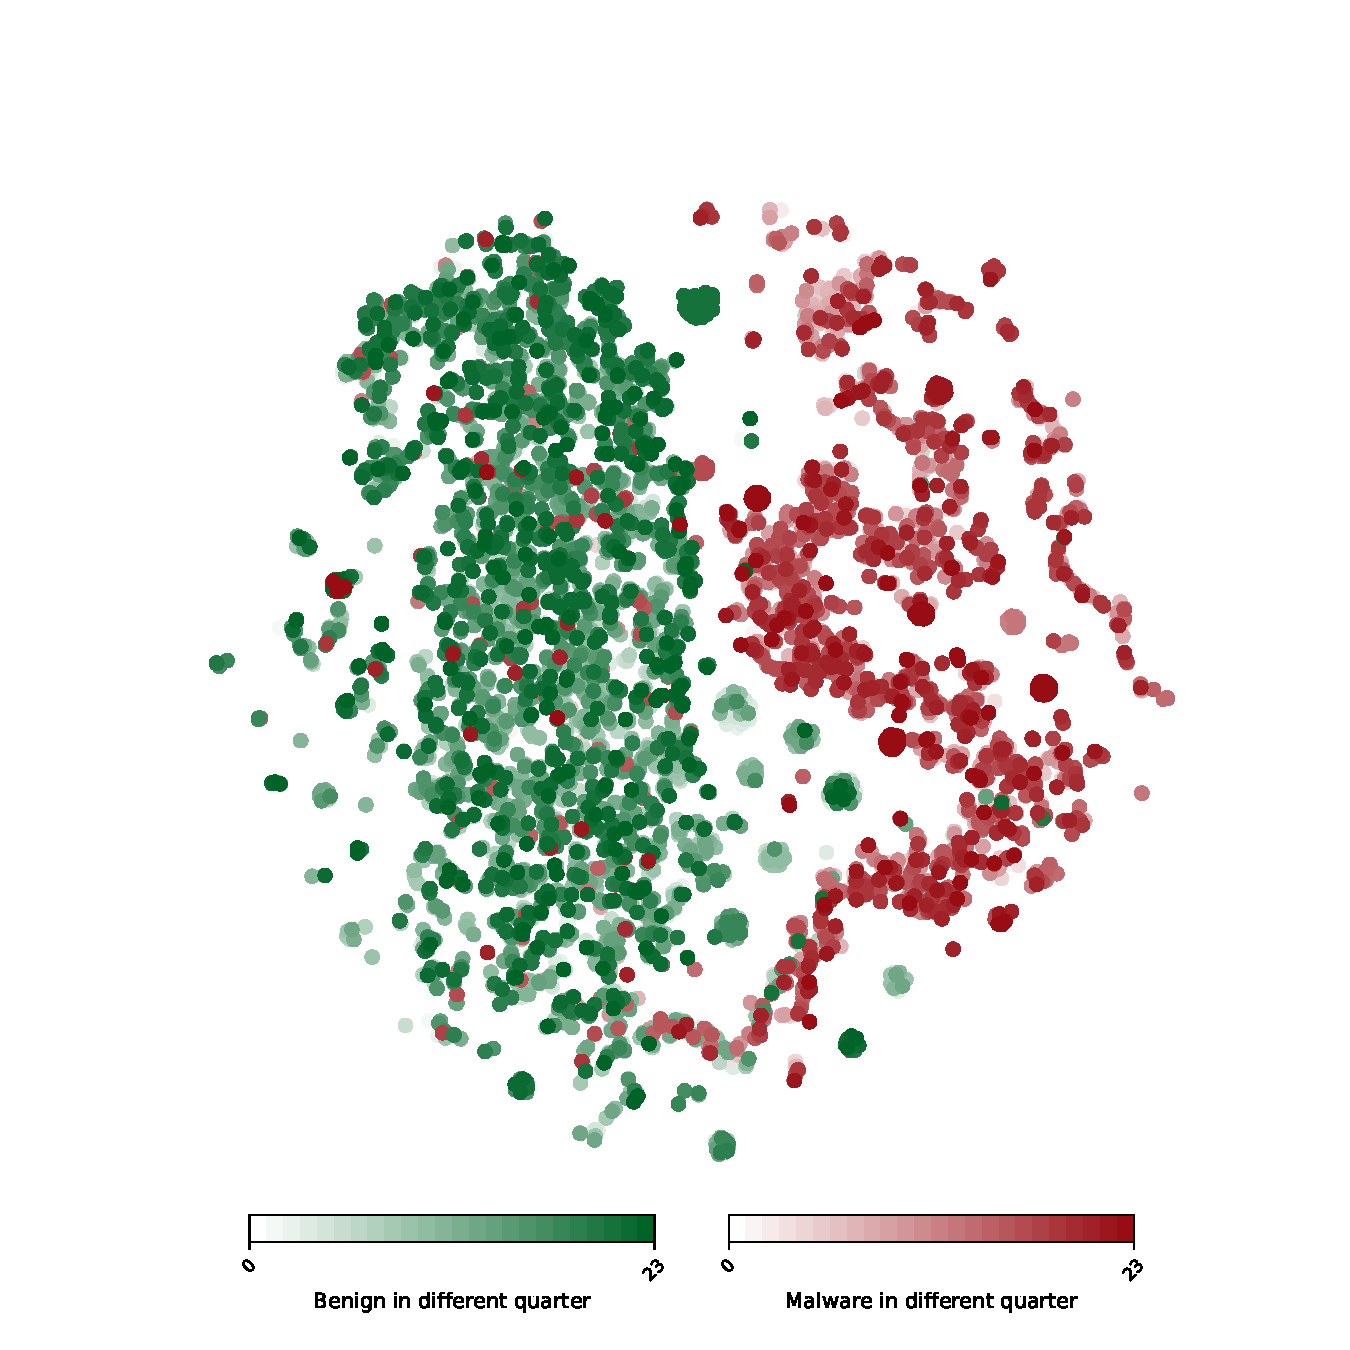
\includegraphics[width=3cm,height=3.5cm]{Graph/Motivation/tsne-APIGraph-v3}
%		\caption{APIGraph}
%		\label{fig::APIGraph PTXY concept drift dataset}
%	\end{subfigure}
%	\hspace{0.5cm}
%	\begin{subfigure}{0.20\textwidth}
%		\centering
%		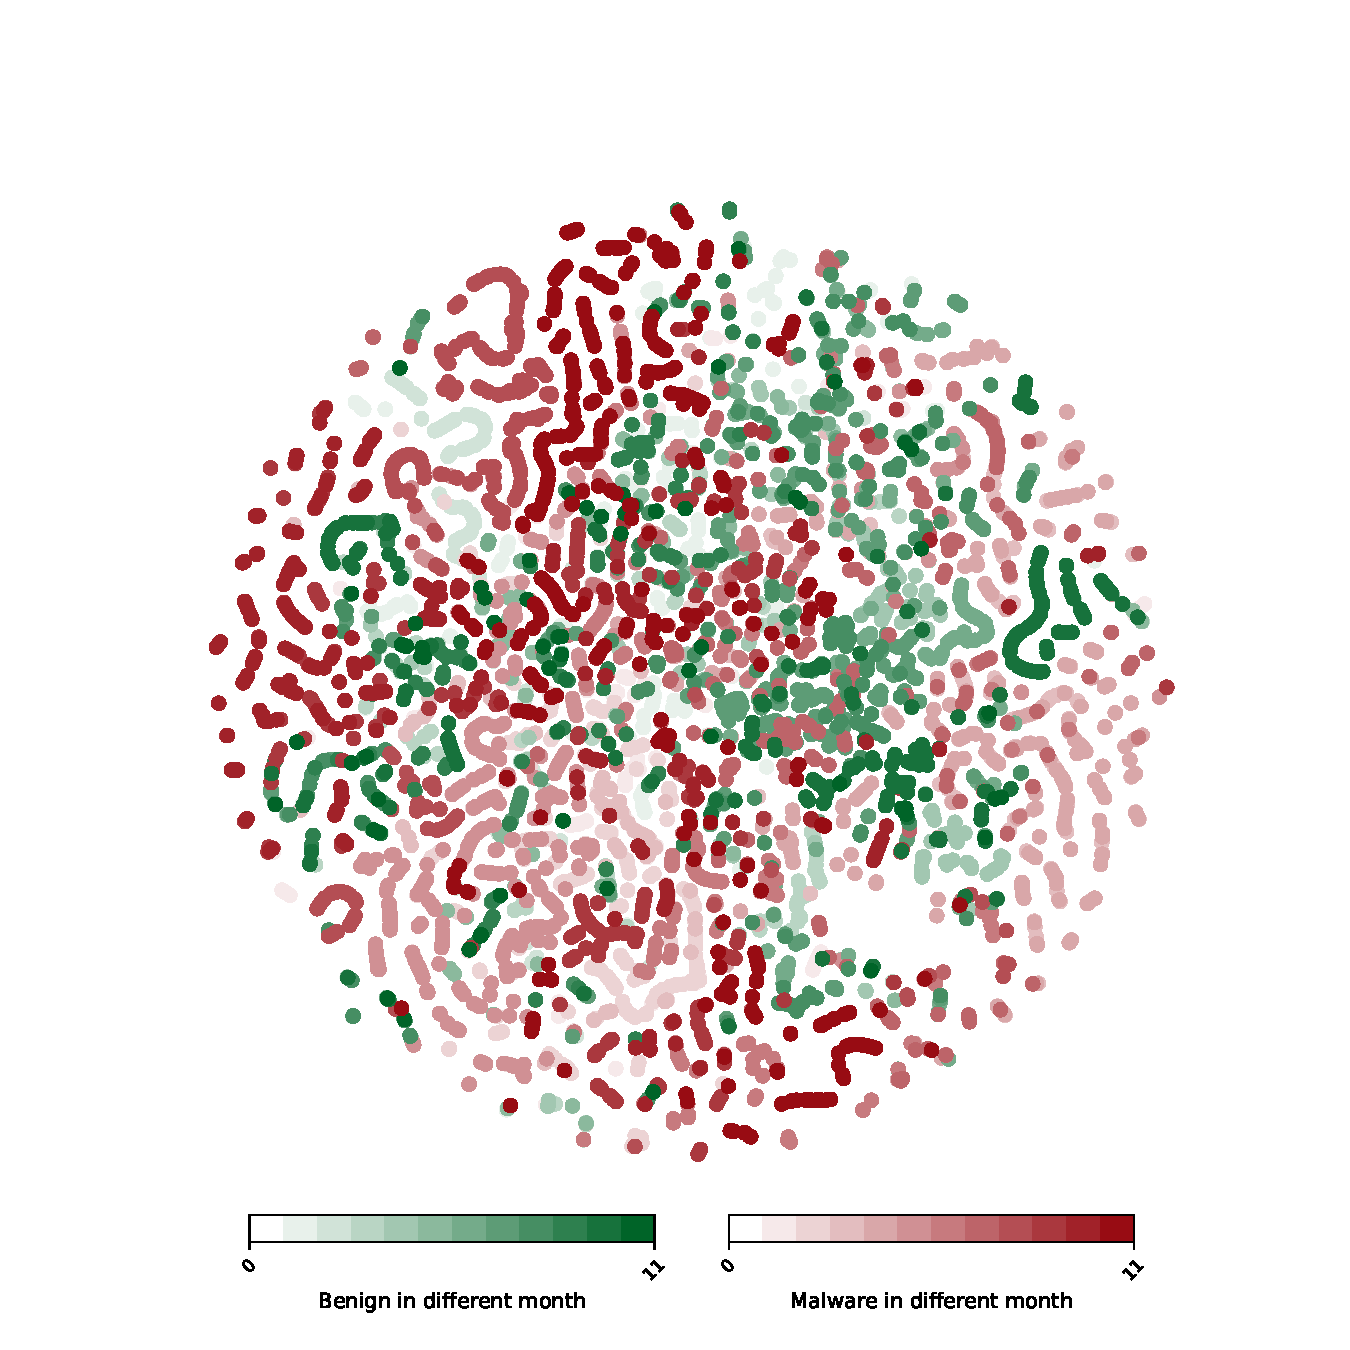
\includegraphics[width=3cm,height=3.5cm]{Graph/Motivation/tsne-BODMAS-v3}
%		\caption{BODMAS}
%		\label{fig::BODMAS PTXY concept drift dataset}
%	\end{subfigure}
%	\caption{T-SNE visualization of $P_{t}(\mathcal{X}|\mathcal{Y})$ concept drift in Android and Windows Malware Datasets}
%	\label{fig:PTXY concept drift in Malware Datasets}
%\end{figure}
%Malware samples may mimic benign characteristics or exhibit distinct malicious features, resulting in continuous changes in the feature distribution, as shown in Figure~\ref{fig:PTXY concept drift in Malware Datasets}.
%Consequently, at the time $t+1$, predicting the shift in $P_{t+1}(\mathcal{X}|\mathcal{Y})$ relative to $P_{t}\mathcal{X}|\mathcal{Y})$ becomes increasingly challenging.
%
%\noindent \textbf{(2) $P_{t}(\mathcal{Y})$ Concept Drift:} 
%Figure~\ref{fig:Attack Motivation-1} illustrates the quarterly distribution of the top 10 categories. 
%Given the significantly higher proportion of benign samples than malware samples, the largest category consists of benign samples, while the remaining nine are malicious families.
%Notably, the distribution shown reflects the label distribution of concept drift samples.
%\begin{figure}[htbp]
%	\centering
%	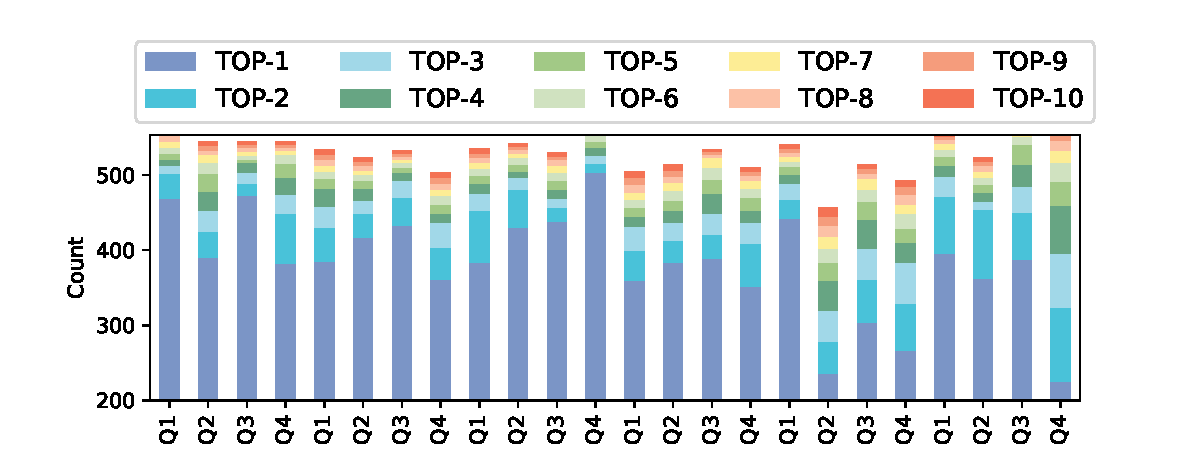
\includegraphics[width=\linewidth,keepaspectratio]{Graph/Evaluation/Figure2.pdf}
%	\caption{$P_{t}(\mathcal{Y})$ Concept Drift during 6 years}
%	\label{fig:Attack Motivation-1}
%\end{figure}
%In practice, the sample selection process is automated, leaving the model owner without access to any information about the distribution of concept drift samples before labeling.
%As a result, filtering poisoned samples becomes significantly more challenging.

\subsection{Shapley Additive Explanations}
\label{Sec: Shapley Additive Explanations}
Recent advances in explainable machine learning have introduced various methods for interpreting the predictions of complex models~\cite{ali2023explainable}.
SHapley Additive exPlanations~\cite{lundberg2017unified} adopt the Shapley value concept from cooperative game theory to assign each feature a contribution score based on its influence on the model's output.
The SHAP framework has been shown to subsume several earlier model explanation techniques~\cite{2021-Usenix-Poisoning-Attack-Explanation-guided-Backdoor}, including LIME~\cite{ribeiro2016should} and Integrated Gradients~\cite{sundararajan2017axiomatic}. 
These model explanation frameworks help determine the importance of each feature value in the model's prediction.
\begin{equation}
	\begin{aligned}
			g(\bm{\mathrm{x}}) = \phi_{0} + \sum_{j=1}^{M} \phi_{j} x_{j}
		\end{aligned}
	\label{SHAP}
\end{equation}
Explanation frameworks construct a surrogate linear model using the input feature vectors and output predictions, leveraging its coefficients to estimate feature importance and direction, as shown in Equation~\ref{SHAP}.
$\bm{\mathrm{x}}$ is the sample, $x_{j}$ is the $j^{th}$ feature for sample $\bm{\mathrm{x}}$, and $\phi_{j}$ is the contribution of feature $x_{j}$ to the model’s prediction.
The SHAP framework stands out by providing theoretical guarantees for calculating feature contributions in a model-agnostic manner.
Recent studies have extended model prediction explanations to include explanations of prediction uncertainty~\cite{NEURIPS2023_16e4be78}.
Motivated by this, we incorporate SHAP-based uncertainty attribution into the design of our poisoning attack against concept drift adaptation methods.

\subsection{Concept Drift Dataset Settings}
\label{Sec: Concept Drift Dataset Settings}
Concept drift datasets have significantly advanced machine learning research due to their rich temporal attribute information.
However, collecting natural concept drift datasets poses challenges, as it incurs significant costs and demands accurate temporal attributes.
Therefore, synthetic datasets are often constructed for experimental evaluation in existing studies, in addition to real-world datasets.

\subsubsection{Synthetic Dataset Construction}
\label{Sec: Synthetic Concept Drift Dataset Construction}
In this experimental evaluation, we constructed synthetic concept drift datasets using a publicly available spam email dataset (SPAM-Email~\cite{2010-Spam-Emali-dataset}) and the MNIST image dataset~\cite{2017-MINIST-dataset}.

\begin{itemize}[leftmargin=*]
	\item[$\bullet$] \textbf{MNIST:} 
	We processed the MNIST handwritten digit dataset to simulate the concept drift phenomenon. 
	Specifically, we selected two clusters of digits, close in the feature space, to represent two classes: digits 3, 5, and 8 (labeled as 0) and digits 4, 7, and 9 (labeled as 1).
	Each digit is treated as a subclass, with new subclasses gradually introduced based on feature similarity to simulate gradual concept drift.
	We randomly selected 30\% of the data from digits 3 and 4 for the initial training set.
	The subsequent five cycles were used as testing periods, each selecting a portion of the unused data as the testing data.
	
	\item[$\bullet$] \textbf{SPAM-Email:} 
	Similar to the concept drift construction in the MNIST dataset, we conducted an in-depth analysis of the original SPAM dataset.
	Using sklearn's k-means algorithm with default parameters, we subdivided legitimate and spam emails into 12 clusters, each representing a distinct subclass.
	Based on this, we designed a concept drift partitioning scheme with nine cycles, each containing 1,036 samples and an approximate 3:1 ratio of legitimate to spam emails.
	To simulate concept drift, we introduced a new subclass of legitimate and spam emails in each cycle while ensuring data from the same subclass appeared in consecutive cycles to reflect emerging trends.
	The first cycle served as the training data, containing one subclass for legitimate emails and one for spam. In subsequent testing cycles, new subclasses were introduced, and the proportions of existing subclasses were adjusted, ensuring at least four subclasses were present in each cycle.
	This approach enabled a smooth evolution of the data distribution over time while ensuring orderly family replacement.
\end{itemize}

\subsection{Training and Testing Data Splits}
\label{Sec: Training and Testing Data Splits}
Most training and testing data partitions are static, with the model trained on the training dataset and evaluated on a fixed testing data.
However, testing data in concept drift scenarios are dynamic and continuously evolving.
Both the distribution and size of the testing data change as time progresses.

\begin{itemize}[leftmargin=*]
	\item[$\bullet$] \textbf{APIGraph:} The APIGraph~\cite{2020-CCS-APIGraph} dataset is trained on data from 2012, with concept drift testing conducted on data from 2013 to 2018, where the data for each year is incrementally released monthly.
	The ratio of legitimate to malicious software for each year is roughly maintained at 9:1, simulating the real-world scenario where legitimate samples significantly outnumber malicious ones.
	Detailed data partitioning is provided in Table~\ref{tab: APIGraph Dataset}.
	
	\item[$\bullet$] \textbf{Androzoo:} The Androzoo\cite{2016-Androzoo} dataset is trained on data from 2017, with concept drift testing conducted on data from 2018 to 2022, where the data for each year is incrementally released monthly.
	The experimental settings for the other datasets are similar to those used for the APIGraph~\cite{2020-CCS-APIGraph} dataset.
	Detailed data partitioning is provided in Table~\ref{tab: Androzoo Dataset}.
	
	\begin{table}[h!]
		\caption{Android Concept Drift Dataset (Androzoo)}
		\label{tab: Androzoo Dataset}
		\setlength{\tabcolsep}{5.8pt}
		\begin{center}
			\scalebox{1.0}{
				\begin{tabular}{cccc}
					\toprule
					\textbf{Year}&\textbf{Malware}&\textbf{Benign}&\textbf{Malware Family}\\
					\midrule
					Train-2017 & 2,108 & 18,972 & 192\\ 
					%				\specialrule{0.05em}{1pt}{1pt}
					Test-2018 (Cycle 1) & 4,625 & 41,625 & 363\\
					%				\specialrule{0.05em}{1pt}{1pt}
					Test-2019 (Cycle 2)& 8,612 & 77,508 & 354\\ 
					%				\specialrule{0.05em}{1pt}{1pt}
					Test-2020 (Cycle 3)& 3,512 & 31,608 & 283\\
					%				\specialrule{0.05em}{1pt}{1pt}
					Test-2021 (Cycle 4)& 4,903 & 44,127 & 256\\
					%				\specialrule{0.05em}{1pt}{1pt}
					Test-2022 (Cycle 5)& 2,814 & 25,326 & 136\\
					\specialrule{0.05em}{1pt}{1pt}
					Total & 26,574 & 239,166 & 1,584\\
					\bottomrule
			\end{tabular}}
		\end{center}
	\end{table}
	
	
	\item[$\bullet$] \textbf{BODMAS:}
	The BODMAS~\cite{2021-PE-malware-dataset} dataset comprises 57,293 malware samples and 77,142 benign samples.
	The malware samples were randomly selected monthly from a security company's internal malware database, and data collection lasted from August 29, 2019, to September 30, 2020.
%	\begin{table}[t]
%		\begin{center}
%			\caption{Windows Malware Concept Drift Dataset} %标题
%			\label{tab: BODMAS Dataset} %表标签
%			\renewcommand{\arraystretch}{0.8}  % 调整该表格的行距
%			\begin{tabular}{cccc} %c的个数表示表的列数
%				\toprule
%				\textbf{Year} & \textbf{Malware} & \textbf{Benign} & \textbf{Malware Family}\\
%				\midrule
%				Train(before 10/19) & 4741 & 17655 & 330\\ 
%				Test-10/19 & 4549 & 3925 & 236 \\
%				Test-11/19 & 2494 & 3718 & 146 \\ 
%				Test-12/19 & 4039 & 6120 & 147 \\ 
%				Test-01/20 & 4510 & 5926 & 183 \\ 
%				Test-02/20 & 4269 & 3703 & 166 \\ 
%				Test-03/20 & 4990 & 3577 & 192 \\ 
%				Test-04/20 & 4640 & 5201 & 162 \\
%				Test-05/20 & 5449 & 6121 & 180 \\
%				Test-06/20 & 4217 & 8182 & 111 \\
%				Test-07/20 & 4995 & 6392 & 144 \\
%				Test-08/20 & 3823 & 2514 & 125 \\
%				Test-09/20 & 4577 & 4198 & 152\\
%				\midrule
%				\textbf{Total} & \textbf{57293} & \textbf{77142} & \textbf{2274} \\
%				\bottomrule
%			\end{tabular}
%		\end{center}
%	\end{table}
	
	\begin{table}[h!]
		\caption{Windows Malware Concept Drift Dataset}
		\label{tab: BODMAS Dataset}
		\setlength{\tabcolsep}{5.8pt}
		\begin{center}
			\scalebox{1.0}{
				\begin{tabular}{cccc}
					\toprule
					\textbf{Year}&\textbf{Malware}&\textbf{Benign} &\textbf{Malware Family} \\
					\midrule
					Train(before 10/19) & 4,741 & 17,655 & 330\\  
					Test-10/19 (Cycle 1) & 4,549 & 3,925 & 236 \\
					Test-11/19 (Cycle 2) & 2,494 & 3,718 & 146 \\
					Test-12/19 (Cycle 3) & 4,039 & 6,120 & 147 \\
					Test-01/20 (Cycle 4) & 4,510 & 5,926 & 183 \\ 
					Test-02/20 (Cycle 5) & 4,269 & 3,703 & 166 \\
					Test-03/20 (Cycle 6) & 4,990 & 3,577 & 192 \\ 
					Test-04/20 (Cycle 7) & 4,640 & 5,201 & 162 \\ 
					Test-05/20 (Cycle 8) & 5,449 & 6,121 & 180 \\ 
					Test-06/20 (Cycle 9) & 4,217 & 8,182 & 111 \\ 
					Test-07/20 (Cycle 10) & 4,995 & 6,392 & 144 \\ 
					Test-08/20 (Cycle 11) & 3,823 & 2,514 & 125 \\
					Test-09/20 (Cycle 12) & 4,577 & 4,198 & 152 \\
					\specialrule{0.05em}{1pt}{1pt}
					\textbf{Total} & \textbf{57,293} & \textbf{77,142} & \textbf{2,274} \\
					\bottomrule
			\end{tabular}}
		\end{center}
	\end{table}
	
	The data collected before October 2019 is used as the initial training data, while the data collected afterward serves as the concept drift testing data, as shown in Table~\ref{tab: BODMAS Dataset}.
	The testing data is evaluated every month.
	
	\item[$\bullet$] \textbf{SPAM-Email:}
	The dataset contains spam and legitimate messages, with a moderate spam ratio of approximately 25\%.
	It includes 9,324 instances and 500 features.
	The initial training data consists of 771 legitimate emails and 265 spam emails.
	Subsequently, 265 new spam emails and 771 legitimate emails are introduced in each of the 8 concept drift testing cycles.
%	\begin{table}[htbp]
%		\begin{center}
%			\caption{Synthetic Concept Drift Dataset for SPAM-Email} %标题
%			\label{tab: Synthetic Concept Drift Dataset for SPAM-Email} %表标签
%			\renewcommand{\arraystretch}{0.8}  % 调整该表格的行距
%			\begin{tabular}{ccc} %c的个数表示表的列数
%				\toprule
%				\textbf{miner} & \textbf{Spam} & \textbf{Legitimate} \\
%				\midrule
%				Train & 265 & 771 \\ 
%				Test-1 & 265 & 771 \\ 
%				Test-2 & 265 & 771 \\ 
%				Test-3 & 265 & 771 \\ 
%				Test-4 & 265 & 771 \\ 
%				Test-5 & 265 & 771 \\ 
%				Test-6 & 265 & 771 \\
%				Test-7 & 265 & 771 \\
%				Test-8 & 265 & 771 \\
%				\midrule
%				\textbf{Total} & \textbf{2387} & \textbf{6937} \\
%				\bottomrule
%			\end{tabular}
%		\end{center}
%	\end{table}
	
		\begin{table}[h!]
		\caption{Synthetic Concept Drift Dataset for SPAM-Email}
		\label{tab: Synthetic Concept Drift Dataset for SPAM-Email}
		\setlength{\tabcolsep}{5.8pt}
		\begin{center}
			\scalebox{1.0}{
				\begin{tabular}{ccc}
					\toprule
					\textbf{miner} & \textbf{Spam} & \textbf{Legitimate} \\
					\midrule
					Train & 265 & 771 \\ 
					Test-1 (Cycle 1) & 265 & 771 \\ 
					Test-2 (Cycle 2) & 265 & 771 \\ 
					Test-3 (Cycle 3) & 265 & 771 \\ 
					Test-4 (Cycle 4) & 265 & 771 \\ 
					Test-5 (Cycle 5) & 265 & 771 \\ 
					Test-6 (Cycle 6) & 265 & 771 \\
					Test-7 (Cycle 7) & 265 & 771 \\
					Test-8 (Cycle 8) & 265 & 771 \\
					\specialrule{0.05em}{1pt}{1pt}
					\textbf{Total} & \textbf{2,387} & \textbf{6,937} \\
					\bottomrule
			\end{tabular}}
		\end{center}
	\end{table}
	
	\item[$\bullet$] \textbf{MNIST:}
	The MNIST dataset contains handwritten digits. 
	3,591 samples were used for training, and 31,860 samples were distributed across 5 concept drift testing cycles.
%	\begin{table}[htbp]
%		\begin{center}
%			\caption{Synthetic Concept Drift Dataset for MNIST} %标题
%			\label{tab: Synthetic Concept Drift Dataset for MNIST} %表标签
%			\renewcommand{\arraystretch}{0.8}  % 调整该表格的行距
%			\begin{tabular}{ccc} %c的个数表示表的列数
%				\toprule
%				\textbf{Year} & \textbf{Label-1} & \textbf{Label-0} \\
%				\midrule
%				Train & 1752 & 1839 \\ 
%				Test-1 & 1752 & 2923 \\ 
%				Test-2 & 2421 & 2852 \\ 
%				Test-3 & 2463 & 2867 \\ 
%				Test-4 & 2734 & 2603 \\ 
%				Test-5 & 6930 & 4315 \\ 
%				\midrule
%				\textbf{Total} & \textbf{18052} & \textbf{17399} \\
%				\bottomrule
%			\end{tabular}
%		\end{center}
%	\end{table}

	\begin{table}[h!]
	\caption{Synthetic Concept Drift Dataset for MNIST}
	\label{tab: Synthetic Concept Drift Dataset for MNIST}
	\setlength{\tabcolsep}{5.8pt}
	\begin{center}
		\scalebox{1.0}{
			\begin{tabular}{ccc}
				\toprule
				\textbf{Year} & \textbf{Label-1} & \textbf{Label-0} \\
				\midrule
				Train & 1,752 & 1,839 \\ 
				Test-1 (Cycle 1) & 1,752 & 2,923 \\ 
				Test-2 (Cycle 2) & 2,421 & 2,852 \\ 
				Test-3 (Cycle 3) & 2,463 & 2,867 \\ 
				Test-4 (Cycle 4) & 2,734 & 2,603 \\ 
				Test-5 (Cycle 5) & 6,930 & 4,315 \\
				\specialrule{0.05em}{1pt}{1pt}
				\textbf{Total} & \textbf{18,052} & \textbf{17,399} \\
				\bottomrule
		\end{tabular}}
	\end{center}
\end{table}

\end{itemize}


%\subsection{Victim Model Settings}
%\label{Sec: Victim Model Settings}
%We adopt commonly used or well-performing architectures from prior research~\cite{2023-Usenix-chenyizhen,2022-SP-Trancending,2021-Usenix-CDAE} in machine learning tasks for the victim model setup. 
%All experiments are conducted on a Windows 11 system with 96GB memory, one Intel® Core™ i7-14700K 3.4GHz CPU, and an NVIDIA GeForce RTX 4080 SUPER (16GB).
%We present the model parameters optimized for respective classification tasks.
%\begin{table}[htbp]
%	\centering
%	\small
%	\caption{Parameters Setting of CDA-AL}
%	\label{tab: Parameter setting of active learning method}
%	%\renewcommand{\arraystretch}{1.2} % 调整单元格高度
%	\begin{tabular}{c|c c}
%		\hline
%		\textbf{Parameter} & \textbf{APIGraph} & \textbf{MNIST}\\ \hline
%		Optimizer  & SGD & ADAM\\ 
%		LR & 0.003 & 0.0004\\ 
%		Batch size & 1024 & 64\\ 
%		Loss & hi-dist-xent & triplet-mse\\ 
%		LR decay & 0.05 & - \\ 
%		Decay epochs & 10,500,10 & -\\
%		Learning epochs & 50 & 5\\ 
%		\hline
%		\textbf{Parameter} & \textbf{BODMAS} & \textbf{SPAM-Email} \\
%		\hline
%		Optimizer & AdamW & AdamW \\ 
%		LR & 0.0004 & 0.0004 \\ 
%		Batch size & 64 & 64 \\ 
%		Loss & BCE & BCE \\ 
%		LR decay & - & - \\ 
%		Decay epochs & - & - \\
%		Learning epochs & 50 & 5\\ 
%	\end{tabular}
%\end{table}
%Table~\ref{tab: Parameter setting of active learning method} summarizes the parameter settings for experiments conducted on four datasets: APIGraph~\cite{2020-CCS-APIGraph}, MNIST~\cite{2017-MINIST-dataset}, BODMAS~\cite{2021-PE-malware-dataset}, and SPAM-Email~\cite{2010-Spam-Emali-dataset}.
%APIGraph: SGD optimizer with a learning rate (LR) of 0.003, batch size 1024, and hi-dist-xent loss function.
%The learning rate decay was set to 0.05 and applied at epochs 10, 500, and 10.
%The model was trained for 50 epochs.
%MNIST: Adam optimizer with an LR of 0.0004, batch size 64, and triplet-my loss function. 
%No learning rate decay was applied, and the model was trained for five epochs.
%BODMAS and SPAM-Email: AdamW optimizer with an LR of 0.0004, batch size 64, and binary cross-entropy (BCE) loss function.
%No learning rate decay was applied.
%The model was trained for 50 epochs on BODMAS and five epochs on SPAM-Email.

	
\begin{figure*}[ht]
	%\setlength{\belowcaptionskip}{-1.5em} % 控制图片标题与后续文本之间的间距
	\centering
	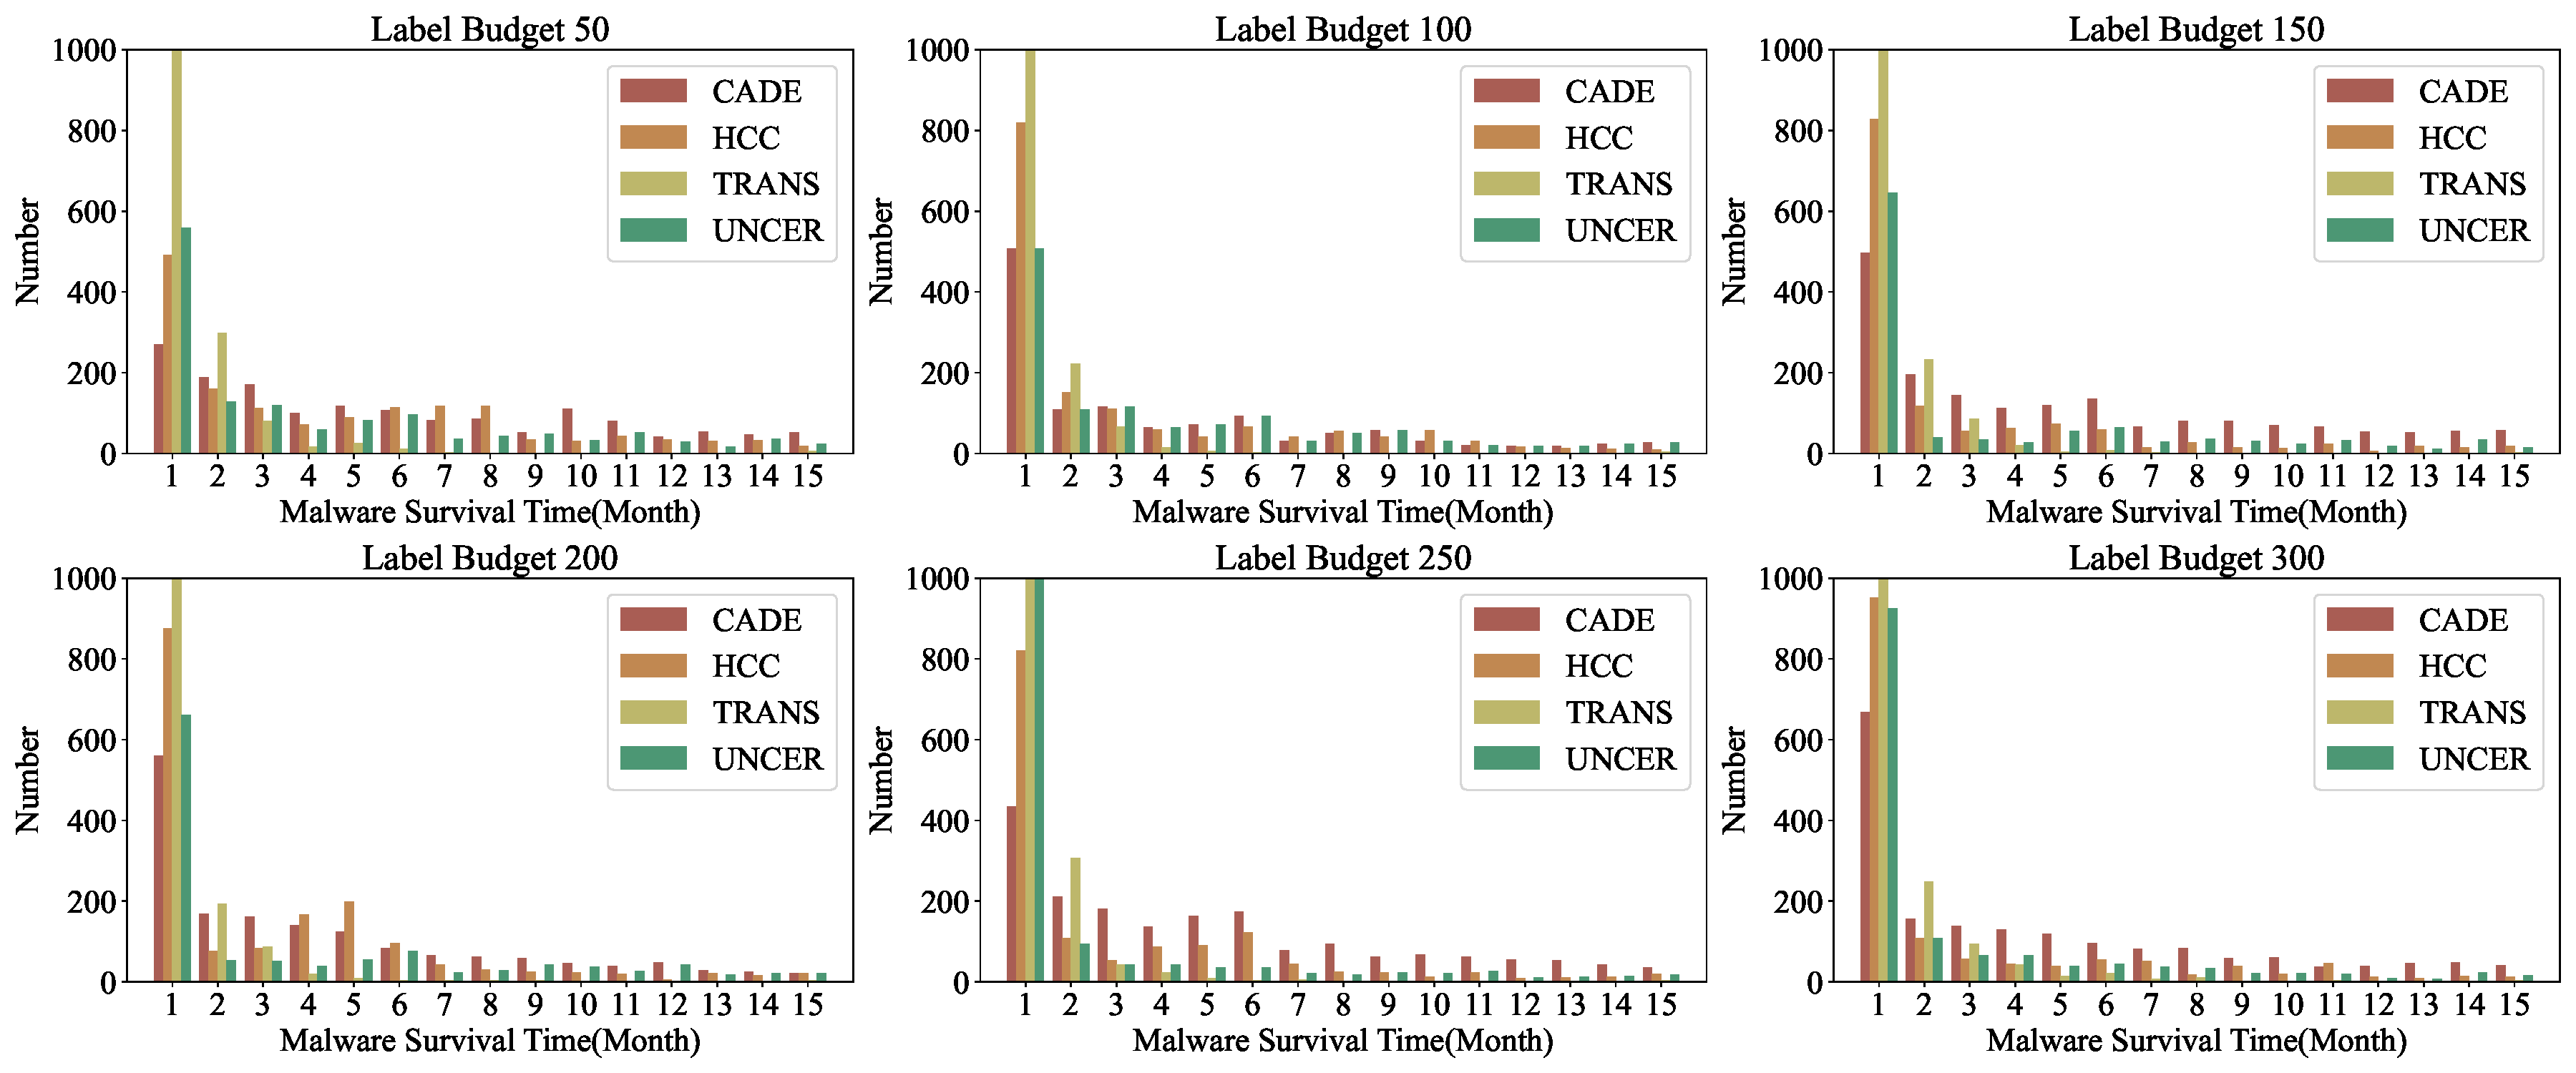
\includegraphics[width=\linewidth,keepaspectratio]{Graph/Appendix/Original_threat_life_cycle_all_budget_0901.pdf}
	\caption{Original misclassification time of attack targets}
	\label{fig: Original survival time of all budget}
\end{figure*}
%\subsection{Concept Drift Adaptation Strategies}
%\label{Sec: Concept Drift Adaptation Strategies}
%
%
%%\textbf{Model Uncertainty.} The core idea of uncertainty measurement~\cite{2023-survey-uncertainty-in-deep-neural-networks} is to detect concept drift based on the output layer of the target model. 
%%The model gives priority to selecting the samples with high uncertainty of the current model for labeling. 
%%A common uncertainty measurement for a neural network is to use one minus the max softmax output of the network.
%
%\noindent \textbf{ (1) Encoder Space Distance (CADE):} CADE~\cite{2021-Usenix-CDAE} trains an encoder through existing labeled data for learning a compressed representation (dimension reduction) of a given input distribution. 
%Then, the newly obtained test samples can be provided to the encoder to obtain the encoder's spatial features. 
%Finally, the distance function can effectively identify concept drift samples far from the existing training dataset.
%
%\noindent \textbf{(2) Credibility and Confidence (TRANS):} Transcending~\cite{2022-SP-Trancending} introduced the thery of conformal prediction~\cite{2005-high-cite-Algorithmic-learning-in-a-random-world} (credibility and confidence) into the field of concept drift adaptation. 
%Given a new test sample, Transcending first computes the non-conformity score of the sample. 
%Then, it computes credibility as the percentage of samples in the calibration set that have higher non-conformity scores than the test sample. 
%Finally, it computes confidence as one minus the credibility of the opposite label. 
%A lower credibility score or a lower confidence score means the test sample is more likely to have drifted.

%\noindent \textbf{(3) Hierarchical Contrastive Loss (HCL):} The method proposed by Chen et al.~\cite{2023-Usenix-chenyizhen} is currently the best-performing strategy in Android malware concept drift adaptation methods. 
%The model consists of two modules. 
%The first module is an encoder and the second module acts as the classifier. 
%In terms of loss function settings, to ensure that the model is robust to concept drift, the training loss of the model is set to the sum of hierarchical contrast loss and classification loss.
%The advantage of this strategy is its provision of finer-grained encoder rules and utilization of similar features among malware families, ultimately enhancing concept drift adaptation performance.


% 2025-Usenix-投稿拒绝
%\section{Original Survival Time of All Label Budget}
%\label{Sec: Original Survival Time of All Label Budget}
%
%\noindent We have analyzed the survival time of new malware under different label budget settings and various concept drift adaptation strategies, as shown in Figure \ref{fig: Original survival time of all budget}. 
%We can observe that the survival time of new malware exhibits a consistent trend, regardless of the label settings and concept drift adaptation strategies.
%Most new malware can survive for 1-5 months under concept drift adaptation strategies, a small portion can survive for more than 5 months, while the survival time of most old malware samples is 0.
%Moreover, most concept drift adaptation strategies face the situation that some new malware survives for more than one year under sufficient label budget (300 samples).
%This phenomenon fully indicates that there is still room for improvement in the performance of the current concept drift adaptation strategies.
%Due to the uneven distribution of survival times for new malware samples under the TRANS concept drift adaptation strategy, the number of samples with survival times of 0-2 months exceeds five times that of samples in other time intervals. 
%Therefore, for the sake of convenient presentation, we have truncated the bar chart representing the 0-2 months survival time samples in the TRANS statistics, while preserving the relative proportions of the overall sample volumes.
%\begin{figure*}[ht!]
%	%\setlength{\belowcaptionskip}{-1em} % 控制图片标题与后续文本之间的间距
%	\centering
%	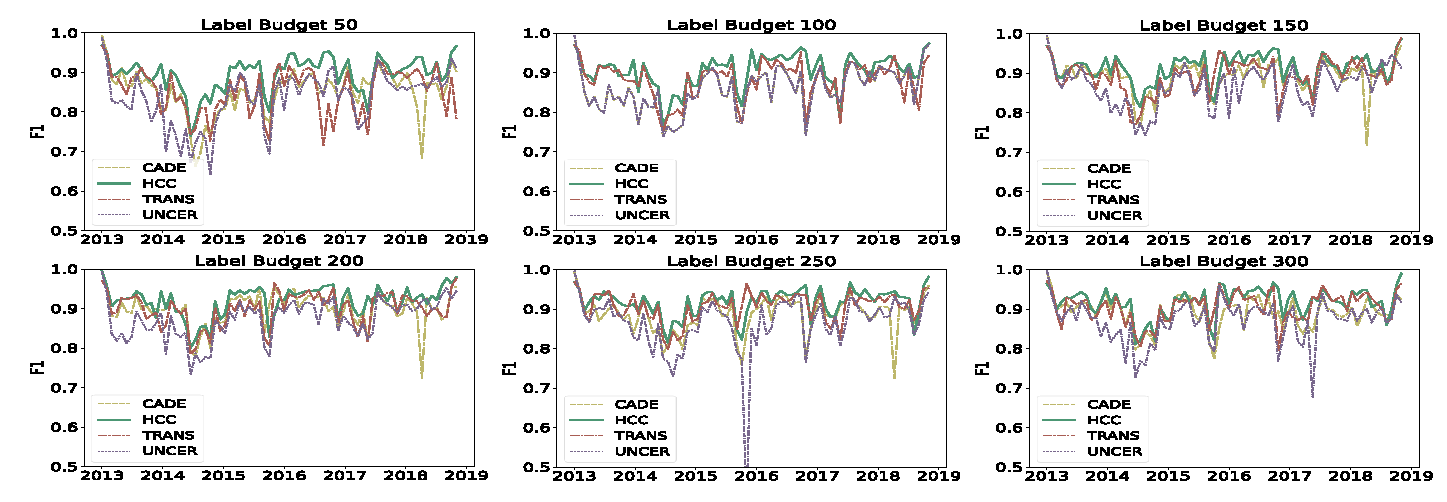
\includegraphics[width=\linewidth,keepaspectratio]{Graph/Appendix/base_performance_allbudget_0830.pdf}
%	\caption{Concept drift adaptation baseline}
%	\label{fig: CDA-AL Baseline}
%\end{figure*}

% \label{sec: Testing of attack overhead in problem space}
% %\vspace{-1em}
% \begin{table}[H]
	% \centering
	% \caption{APK obfuscation time}
	% %\renewcommand{\arraystretch}{0.8}  % 调整该表格的行距
	% \label{tab: APK obfuscation time}
	% \begin{tabular}{c|c|c|c}
		% \toprule
		% \textbf{APK} & \textbf{Size(MB)} & \textbf{Category} & \textbf{Obfuscation} \\
		% \midrule
		% \textbf{JD} & 97.59 & shopping & 54.95s \\
		% \textbf{Taobao} & 57.03 & shopping & 78.98s \\
		% \textbf{Little Red Book} & 162.99 & social & 178.68s \\
		% \textbf{Google} & 315.67 & tool & 93.32s \\
		% \textbf{Wang VPN} & 45.51 & tool & 14.91s \\
		% \textbf{WeChat} & 264.04 & communication & 136.76s \\
		% \midrule
		% \textbf{Average} & 199.72 & - & 90.72s \\
		% \bottomrule
		% \end{tabular}
	% \end{table}

% 这个先不说了
% \textbf{Feature Space Inverse Mapping:} In the end, we need to show that the features corresponding to the poison samples must have corresponding Android applications in the problem space. Since an attack seed sample is an object in the problem space that meets semantic requirements, and the poison samples are single-bit flip variants of the attack seed sample in the feature space, so they also meet semantic requirements in the problem space. For feature spaces such as the APIGraph dataset and the Androzoo dataset, a single transformation means an increase or decrease in an API call or permission declaration. 

%\section{Concept Drift Adaptation Strategy Settings}
%\label{sec: Concept Drift Adaptation Strategy Settings}
%\noindent It is not enough to just enumerate the model structures and concept drift adaptation strategies. 
%What is more critical is to combine them. 
%Our combination follows the principle of optimal configuration. 
%For each target model structure, we select the corresponding concept drift adaptation strategy based on the optimal combination method in existing research methods.
%The last setting about the concept drift adaptation strategy is the initial state of the target model. 
%Our setting in this study is to train the initial data for 1 year, then conduct \pandora attack verification, and use the monthly time window to evaluate and verify the effectiveness of the attack.
%The final combination is shown in Table \ref{tab: Combination of Model Structure and CDA-Strategy}.

%\section{Concept Drift Adaptation Baseline}
%\label{sec: CDA-AL Baseline}
%\noindent We conduct baseline tests on the performance of current mainstream concept drift adaptation methods on the APIGraph~\cite{2020-CCS-APIGraph} and CDAMAL\footnote{\url{https://anonymous.4open.science/r/Denial-of-Concept-Drift-Adaptation-Contribution-343C}} datasets, and the test results are shown in the Figure \ref{fig: CDA-AL Baseline}. 
%We run all experiments on a Win11 with 96GB memory, 1 Intel (R) Core (TM)i7-14700K 3.4GHz CPU and one NVIDIA GeForce RTX 4080 SUPER (16GB). 
%\begin{comment}
%	\begin{table}[h]
%		\centering
%		\small
%		\caption{Parameter setting of active learning method}
%		\label{tab: Parameter setting of active learning method}
%		%\renewcommand{\arraystretch}{1.2} % 调整单元格高度
%		\begin{tabular}{c|c c}
%			% \hline
%			\multirow{2}{*}{Parameter} & \multicolumn{2}{c}{Method} \\ \cline{2-3} 
%			& \textbf{HCL} & \textbf{CADE}\\ \hline
%			Optimizer  & SGD & ADAM\\ 
%			LR & 0.003 & 0.0001\\ 
%			Batch size & 1024 & 32\\ 
%			Loss & hi-dist-xent & triplet-mse\\ 
%			LR decay & 0.05 & 1\\ 
%			Decay epochs & 10,500,10 & 10,500,10\\
%			Scheduler & step & cosine\\ 
%			Learning epochs & 50 & 50\\ 
%			\hline
%			Parameter & \textbf{TRANS} & \textbf{UNC} \\
%			\hline
%			Optimizer & SGD & SGD \\ 
%			LR & 0.003 & 0.003 \\ 
%			Batch size & 512 & 1024 \\ 
%			Loss & hi-dist & hi-dist-xent \\ 
%			LR decay & 0.95 & 0.95 \\ 
%			Decay epochs & 10,500,10 & 30,1000,30 \\
%			Scheduler & step & step \\ 
%			Learning epochs & 50 & 50\\ 
%		\end{tabular}
%	\end{table}
%\end{comment}
%Here, we offer a concise overview of the hyperparameter configurations. 
%We utilize the SGD optimizer for HCL, TRANS, and UNC while employing the ADAM optimizer for CADE. 
%For the loss functions, TRANS uses the Hierarchical Distance loss function, CADE uses the Triplet Mean Squared Error loss function, and HCL and UNC employe the Hierarchical Distance Cross-Entropy loss function. 
%The total number of training epochs is set to 50 for all four methods.
%More detailed hyperparameter settings are shown in Table \ref{tab: Parameter setting of active learning method}.
%In this study, we test four types of current mainstream excellent Android malware detection models~\cite{2020-CCS-APIGraph,2023-TIFS-Federated-Android-Malware-ResNet,2023-Usenix-chenyizhen}, and the obtained concept drift detection data is shown in Figure \ref{fig: CDA-AL Baseline}.
%It can be observed that the higher the label budget setting is, the better the performance of the concept drift adaptation method becomes.
%Moreover, the latest concept drift adaptation method (HCL~\cite{2023-Usenix-chenyizhen}) demonstrates performance advantage over the existing methods (TRANS~\cite{2022-SP-Trancending},CADE~\cite{2021-Usenix-CDAE},UNCER~\cite{2023-survey-uncertainty-in-deep-neural-networks}).
%We notice that the performance of existing concept drift adaptation strategies is unstable, and even the optimal HCL method has performance fluctuations.
%The instability also inspires the research on the security of concept drift adaptation strategies in our study.

%As can be seen from the figure, after 6 years, the detector's F1 score index averaged 0.73 per month, a decrease of 0.26 compared to the initial month, and the lowest point dropped to 0.32 in November 2015, with an FNR as high as 77.66\%.

% \begin{table}[h]
	% \centering
	% \small
	% \caption{Parameter setting of active learning method}
	% \label{tab: Parameter setting of active learning method}
	% %\renewcommand{\arraystretch}{1.2} % 调整单元格高度
	% \begin{tabular}{c|c c c c }
		% % \hline
		% \multirow{2}{*}{\textbf{Parameter}} & \multicolumn{4}{c}{\textbf{Method}} \\ \cline{2-5} 
		%  & \textbf{HCC} & \textbf{CADE} & \textbf{TRANS} & \textbf{UNC} \\ \hline
		% \textbf{Optimizer}  & SGD & ADAM & SGD & SGD \\ 
		% \textbf{LR} & 0.003 & 0.0001 & 0.003 & 0.003 \\ 
		% \textbf{Batch size} & 1024 & 32 & 512 & 1024 \\ 
		% \textbf{Loss} & hi-dist-xent & triplet-mse & hi-dist & hi-dist-xent \\ 
		% \textbf{LR decay} & 0.05 & 1 & 0.95 & 0.95 \\ 
		% \textbf{Decay epochs} & 10,500,10 & 10,500,10 & 10,500,10 & 30,1000,30 \\
		% \textbf{Scheduler} & step & cosine & step & step \\ 
		% \textbf{learning epochs} & 50 & 50 & 50 & 50 \\ 
		% \end{tabular}
	% \end{table}



%\section{Freeze Attack Strategy}
%\label{Sec: Attack Value Unstable}
%%\begin{figure}[h]
%%	%\setlength{\belowcaptionskip}{-1em} % 控制图片标题与后续文本之间的间距
%%	\centering    
%%	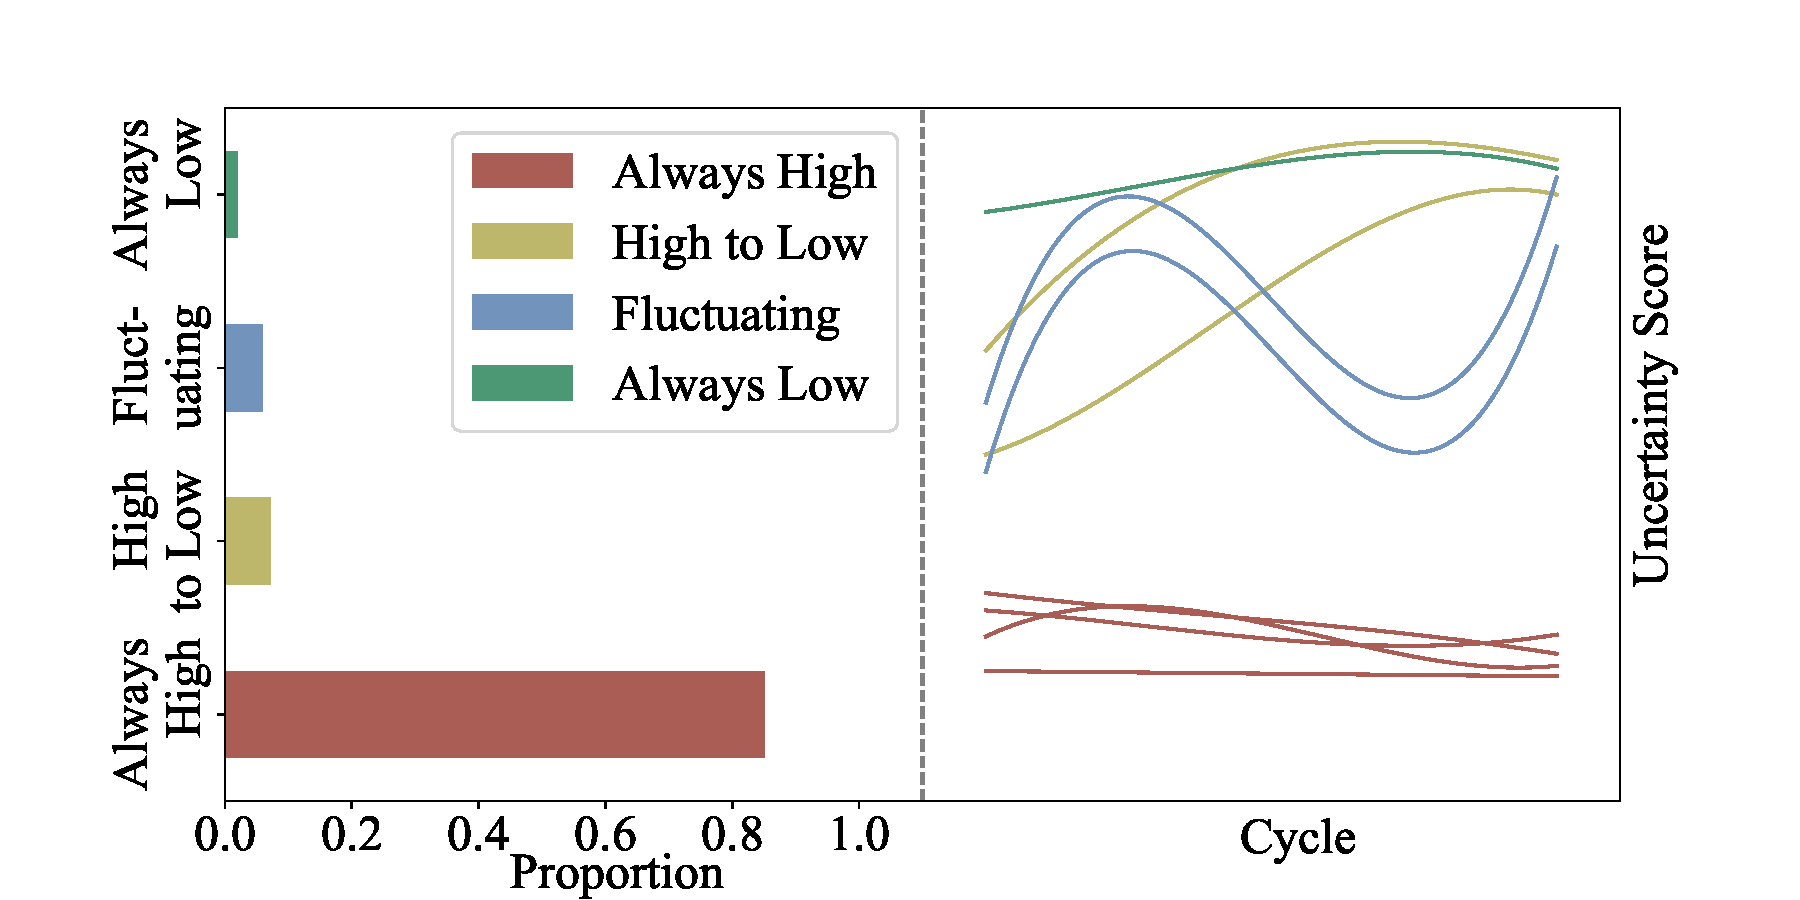
\includegraphics[width=\linewidth,keepaspectratio]{Graph/Appendix/attack_value_change_0830.pdf}       	
%%	\caption{Attack value unstable}
%%	\label{fig: Attack Value Unstable}
%%\end{figure}
%%%It is important to note that the \pandora attack framework is an automated attack framework, which needs to continuously generate poisoned samples in each model cycle.
%%Therefore, the malware attack value assessment module and the survival time prolongation module need to be integrated with each model cycle. 
%
%\noindent We observe that the attack value of new high uncertainty malware in the initial model cycle also exhibits instability in subsequent model cycles.
%%, as shown in Figure \ref{fig: Attack Value Unstable}. 
%While 85\% of the samples maintain a high attack value in the subsequent cycles, nearly 15\% of the samples experience fluctuations in their attack value.
%Specifically, the attack value of the samples may oscillate between high and low values, or it may shift from high value to low value. 
%To ensure the consistency of attack effectiveness across consecutive model cycles, we employ freeze attacks during the low attack value model cycles of new malware. 
%Freeze attack involves selecting benign poisoned seed samples with the highest uncertainty score. 
%During the poisoned sample generation phase, data augmentation based on sample replication strategies is applied to produce a batch of attack samples.


% 相关工作的这部分不放正文了,信息量太少,都是前面说过的东西
% \textbf{Concept Drift Adaptation.} Currently, researchers believe that the phenomenon of concept drift is the main reason affecting the survival time of new malware. Researchers have proposed a series of methods~\cite{2023-Usenix-chenyizhen,2022-SP-Trancending,2021-Usenix-CDAE,2017-Usenix-Transcend} to detect concept drift samples and optimize models. Furthermore, Yiling He et al.~\cite{2024-arxiv-Going-Proactive-and-Explanatory-Against-Malware-Concept-Drift} have proposed DREAM, a method that can effectively enhance the accuracy of drift detection and reduce the cost of manual analysis. Our work primarily focuses on detecting concept drift, as this phase serves as the foundation for subsequent stages. While existing research has mainly concentrated on optimizing the performance of adaptation methods for concept drift, our emphasis lies on its security.
\subsection{Model parameters}
\label{Sec: Model parameters}
APIGraph: The model was trained for 50 epochs using the SGD optimizer with a learning rate (LR) of 0.003, batch size of 1024, and hi-dist-xent loss.
A learning rate decay factor of 0.05 was applied every 10 epochs starting from epoch 10.
MNIST: The model was trained for 5 epochs with the Adam optimizer (LR = 0.0004), batch size of 64, and triplet-my loss. No learning rate decay was applied.
BODMAS and SPAM-Email: Both models used the AdamW optimizer (LR = 0.0004), batch size of 64, and binary cross-entropy (BCE) loss.
BODMAS was trained for 50 epochs and SPAM-Email for 5 epochs. No learning rate decay was applied.

\subsection{Attack Targets List}
\label{Sec: Attack Target List}
The experimental evaluation was conducted under various attack targets configurations to validate the effectiveness of the proposed method and to analyze factors influencing attack success.
The detailed information is as follows.

\begin{itemize}[leftmargin=*]
	
	\item[$\bullet$] \textbf{Single-Target Attack:} 
	We followed two principles when selecting attack targets.
	First, the attack targets must not be included in the training set.
	Second, the attack targets is misclassified during the month it appears.
	This indicates that the attack target is a newly emerging concept drift sample in the testing phase rather than a simple modification of existing samples in the training data.
	Moreover, this also prevents situations where the attack targets lack sufficient attack value.
	
	\item[$\bullet$] \textbf{Multi-Target Attack:} 
	The attack targets for multi-target attacks are composed of multiple single-attack targets that emerge simultaneously.
	The targets of APIGraph are detailed in Table~\ref{tab: Attack Target for Multi-target Attack}.
	The concept drift adaptation associated with the attack target spans five years.
	For other datasets, the multi-target attack is conducted over the entire set of attack targets.
	\begin{table}[ht!]
		\begin{center}
			\caption{Attack Target for Multi-target Attack} %标题
			\label{tab: Attack Target for Multi-target Attack} %表标签
			\renewcommand{\arraystretch}{0.8}  % 调整该表格的行距
			\begin{tabular}{ccc} %c的个数表示表的列数
				\toprule
				\textbf{Month} & \textbf{Type} & \textbf{Family} \\
				\midrule
				\multirow{6}{*}{2013-09} & \multirow{3}{*}{Non-Target} 	& ansca \\ 
				&	& cardserv \\ 
				&	& svpeng  \\ \cline{2-3}
				& \multirow{3}{*}{Target} 	& mecor  \\
				&	& smforw \\
				&	& vietsms \\
				\midrule
				\multirow{5}{*}{2014-05} & \multirow{3}{*}{Non-Target} 	& gabas \\ 
				&	& simplocker \\ 
				&	& smssend \\ \cline{2-3}
				& \multirow{2}{*}{Target} 	& mecor  \\
				&	& svpeng  \\ 
				\midrule
				\multirow{6}{*}{2014-06} & \multirow{4}{*}{Non-Target} 	& chyapo \\ 
				&	& pletor \\
				&	& spyware \\
				&   & tebak   \\ \cline{2-3}
				& \multirow{2}{*}{Target} 	& mecor \\
				&   & adflex  \\
				\midrule
				\multirow{5}{*}{2014-09} & \multirow{3}{*}{Non-Target} 	& fobus \\ 
				&	& gamecheater \\
				&   & ransomware  \\ \cline{2-3}
				& \multirow{2}{*}{Target} 	& mecor \\
				&   & spyware  \\
				\midrule
				\multirow{5}{*}{2014-10} & \multirow{3}{*}{Non-Target} 	& fakebank \\ 
				&	& systemmonitor \\
				&   & webapp  \\ \cline{2-3}
				& \multirow{2}{*}{Target} 	& airpush \\
				&   & mecor  \\
				\midrule
				\multirow{5}{*}{2015-05} & \multirow{3}{*}{Non-Target} 	& adflex \\ 
				&	& kalfere \\
				&   & styricka  \\ \cline{2-3}
				& \multirow{2}{*}{Target} 	& mobidash \\
				&   & vnapstore  \\
				\midrule
				\multirow{4}{*}{2016-07} & \multirow{1}{*}{Non-Target} 	& clicks \\  \cline{2-3}
				& \multirow{3}{*}{Target} 	& adflex \\
				&   & blouns  \\
				&   & mspy    \\
				\midrule
				\multirow{3}{*}{2017-01} & \multirow{1}{*}{Non-Target} 	& mobidash \\  \cline{2-3}
				& \multirow{2}{*}{Target} 	& batmob \\
				&   & kalfere  \\
				\midrule
			\end{tabular}
		\end{center}
	\end{table}
	
	%\noindent \textbf{(3) Dynamic Switching Between Different Attack Target Configurations:} 
	%The target selection rules are the same as those for the multi-target attack scenario.
	%The attack targets are detailed in Table~\ref{tab: Attack Target for Dynamic Switching}.
	%\begin{table}[htbp]
	%	\begin{center}
		%		\caption{Attack Target for Dynamic Switching} %标题
		%		\label{tab: Attack Target for Dynamic Switching} %表标签
		%		\renewcommand{\arraystretch}{0.8}  % 调整该表格的行距
		%		\begin{tabular}{cc|cc} %c的个数表示表的列数
			%			\toprule
			%			\textbf{Month} & \textbf{Family} & \textbf{Month} & \textbf{Family} \\
			%			\midrule
			%			\multirow{5}{*}{2014-09} & mecor & \multirow{5}{*}{2015-01} & airpush\\ 
			%									 & spyware &  & mobidash \\ 
			%									 & gamecheater &  & svpeng \\ 
			%									 & ransomware &  & kemoge \\ 
			%									 & fobus &  & gorpo \\ 
			%			\midrule
			%			\multirow{4}{*}{2016-07} & clicks & \multirow{4}{*}{2018-01} & itracker\\ 
			%									& adflex &  & faketoken \\ 
			%									& blouns &  & clicks \\ 
			%									& mspy &  & miner \\ 
			%			\midrule
			%		\end{tabular}
		%	\end{center}
	%\end{table}
\end{itemize}



\subsection{Attack Targets Initial Misclassification Time}
\label{Sec: Attack Target Initial Survival Time (APIGraph)}
Since the effectiveness of the \pandora is defined by prolonging the misclassification duration of the original attack targets, it is essential to test the misclassification duration of the attack targets in the absence of any attacks.
We analyzed the misclassification time of malware under different labeling budget settings and concept drift adaptation strategies, as shown in Figure~\ref{fig: Original survival time of all budget}.
Most malware is misclassified for 1-5 months under CDA-AL, while a small portion survives for over 5 months.
The \pandora aims to extend the misclassification duration of targeted samples. 
Therefore, we selected all malware samples in the testing phase with a misclassification duration of 15 months or less as attack targets.
We performed similar operations on the other three datasets to extract the original misclassification times of the attack targets.

%\section{Attack Method Details}
%\label{Sec: Attack Method Details}

%\subsection{The Alignability of Real-World Data}
%\label{Sec: Real-World Alignment with the Gray-Box Assumption}
%% 代理模型数据对齐相关分析
%The alignment degree between the data collection capabilities of the surrogate model and the victim model is a critical factor influencing the surrogate model's ability to simulate the victim model's inference behavior.
%However, we find that in concept drift adaptation systems for sensitive domains (e.g., VirusTotal), platform maintainers often utilize hash functions as sample indices to enable precise matching during the sample query process.
%Although exact matching improves the performance of concept drift adaptation, it inadvertently aids attackers in aligning data more effectively, allowing them to build more accurate surrogate models.
%This alignment, in turn, enhances the efficiency of \pandora attacks.
%% 现实世界代理模型黑盒与灰盒相关分析
%In black-box settings, attackers must construct surrogate models to estimate sample uncertainties, which increases their costs.
%Conversely, gray-box settings eliminate the need for surrogate models, significantly lowering attack expenses.
%Moreover, real-world machine learning systems~\cite{Baidu-ImageRecognition} provide confidence information (indicating sample uncertainty) to enhance user experience.
%This practice aligns with the gray-box assumption, making it more applicable to practical scenarios while further reducing the cost of \pandora attacks.
%The alignment between the data collection capabilities of the surrogate model and the victim model is a critical factor in simulating the victim model's inference behavior. 
%Specifically, in concept drift adaptation systems for sensitive domains (e.g., VirusTotal~\ref{Virustotaluploadinterface}), platform maintainers often use hash functions to index samples, enabling precise matching during the query process. 
%While this enhances adaptation performance, it also inadvertently aids attackers in aligning data more effectively, allowing them to build more accurate surrogate models and thereby increasing the efficiency of \pandora attacks.
%Moreover, real-world machine learning systems~\cite{Baidu-ImageRecognition} often provide confidence scores to enhance user experience. 
%This practice aligns with the gray-box assumption, making it highly relevant to practical scenarios and further lowering the cost of \pandora attacks.
%The alignment between the surrogate and victim models' data collection capabilities is critical in simulating the victim model's inference behaviour.
%Specifically, in concept drift adaptation systems for sensitive domains (e.g., VirusTotal~\cite{Virustotaluploadinterface}), platform maintainers often use hash functions to index samples, facilitating precise matching during the query process. While this improves adaptation performance, it also inadvertently helps attackers align data more effectively, enabling the construction of accurate surrogate models and enhancing \pandora attack efficiency.
%Moreover, real-world machine learning systems~\cite{Baidu-ImageRecognition} often provide confidence scores to improve user experience. 
%
%\noindent \textbf{In summary:} Real-world scenarios align more closely with the gray-box assumption, making \pandora attacks highly applicable in practical settings while simultaneously reducing their costs.

%\begin{table}[t]
%	\caption{Problem-Space Perturbation Operations} %标题
%%	\label{tab: List of Problem Space Perturbation Operations} %表标签
%	\centering
%	\renewcommand{\arraystretch}{0.95}  % 调整表格的行距
%	\small
%	\begin{tabular}{|>{\centering\arraybackslash}p{1.2cm}|>{\centering\arraybackslash}p{6.0cm}|}
%		\hline
%		\textbf{Dataset}                   & \textbf{Perturbation Operations} ($\alpha$) \\ \hline
%		\multirow{3}{*}{APIGraph} & Rename method names to meaningless identifiers            \\ \cline{2-2} 
%		& Modify image and other resource files     \\ \cline{2-2} 
%		&Transform complex control structures into simpler ones    \\ \hline
%		\multirow{3}{*}{BODMAS}   & Modify the system API function names                       \\ \cline{2-2} 
%		& Move variables to the header structure fields            \\ \cline{2-2} 
%		& Dynamically adjust the size of the DOS STUB space        \\ \hline
%		\multirow{3}{*}{MNIST}   & Add Gaussian noise to the image pixels                      \\ \cline{2-2} 
%		&  Perform geometric transformations, such as rotation                    \\ \cline{2-2} 
%		& Apply sharpening to enhance the edges of the image                        \\ \hline
%		\multirow{3}{*}{SPAM}     &  Remove non-essential words                       \\ \cline{2-2} 
%		&  Split long sentences into shorter ones                      \\ \cline{2-2} 
%		& Insert random symbols or additional spaces                        \\ \hline
%	\end{tabular}
%\end{table}

%\subsection{Attack Negotiation Details}
%\label{Sec: Attack Negotiation Details}
%% 攻击协商协议细节
%To further elaborate, the following details describe the attack negotiation process and its implementation.
%At time $t$, attacker $\mathcal{A}_{m}$ begins by evaluating the potential attack value of their target sample $x_{tar}^{m}$, as shown in Step-II-D (Figure~\ref{fig: Attack Negotiation}).
%This assessment is based on two key indicators: the predicted pseudo label $\overline{y}_{tar}^{m}$ of the attack target $x_{tar}^{m}$, generated by the surrogate model $S_{t}$, and the uncertainty score $u_{tar}^{m}$.
%The pseudo labels $\overline{y}_{tar}^{m}$ reflect the survival probability of the target sample $x_{tar}^{m}$ under the current model state at time $t$.
%Simultaneously, the uncertainty score $u_{tar}^{m}$ quantifies the likelihood that $x_{tar}^{m}$ will be flagged for manual analysis based on the label budget threshold $\beta$.
%Only samples with uncertainty $u_{tar}^{m}$ below the threshold $\beta$ are considered valuable for the attack.
%If a target sample $x_{tar}^{m}$ is submitted for manual analysis, the victim model will learn the ground truth label ${y}_{tar}^{m}$, thereby neutralizing the attack’s effect.
%Attack targets that are misclassified $\left( y_{tar}^{m} \ne \overline{y}_{tar}^{m} \right)$ under the current model state and are resistant to manual analysis hold attack value.
%Conversely, if a target does not meet these criteria, the attacker does not have sufficient time to execute a data poisoning attack effectively.
%As a result, such samples are either immediately detected as correct label during the testing cycle in which they appear or, following manual analysis, are added to the detection system's blacklist.
%For targets lacking attack value, the attacker withdraws from the current attack negotiation to conserve resources.
%To validate the effectiveness of the attack value evaluation module, we also conducted ablation experiments detailed in Appendix~\ref{Sec: Other Attack Influencing Factors under TPA}.
%After each attacker identifies their high-value targets $x_{tar}^{m}$, they proceed to negotiate the attack targets, as illustrated in Step-III to Step-VII (Figure~\ref{fig: Attack Negotiation}).
%Steps III to VII follow the standard Millionaire’s Protocol algorithm, which can also be replaced in practice with any more efficient cryptographic protocol providing equivalent functionality.

%\subsection{Side Effects of Problem-Space Perturbation}
%\label{Sec: Side Effects of Problem Space Perturbation}
%\begin{table}[htbp]
%	\caption{Problem-Space Perturbation Operations} %标题
%	\label{tab: List of Problem Space Perturbation Operations} %表标签
%	\centering
%	\renewcommand{\arraystretch}{0.9}  % 调整表格的行距
%	\small
%	\begin{tabular}{|c|c|}
%		\hline
%		\textbf{Dataset}                   & \textbf{Perturbation Operations} ($\alpha$) \\ \hline
%		\multirow{3}{*}{APIGraph} & Rename method names to meaningless identifiers            \\ \cline{2-2} 
%		& Modify image and other resource files     \\ \cline{2-2} 
%		&Transform complex control structures into simpler ones    \\ \hline
%		\multirow{3}{*}{BODMAS}   & Modify the system API function names                       \\ \cline{2-2} 
%		& Move variables to the header structure fields            \\ \cline{2-2} 
%		& Dynamically adjust the size of the DOS STUB space        \\ \hline
%		\multirow{3}{*}{MNIST}   & Add Gaussian noise to the image pixels                      \\ \cline{2-2} 
%		&  Perform geometric transformations, such as rotation                    \\ \cline{2-2} 
%		& Apply sharpening to enhance the edges of the image                        \\ \hline
%		\multirow{3}{*}{SPAM}     &  Remove non-essential words                       \\ \cline{2-2} 
%		&  Split long sentences into shorter ones                      \\ \cline{2-2} 
%		& Insert random symbols or additional spaces                        \\ \hline
%	\end{tabular}
%\end{table}
%%%%%%%%%%%%%%%
%As shown in Section~\ref{Sec: Poisoned Sample Generation}, under the condition of maintaining consistency in the feature space, the attacker generates poisoned samples using perturbations in the problem space. 
%For data domains such as images and text, the goal of poisoned samples is to reduce the performance of the victim model.
%Therefore, the attack is considered adequate as long as the poisoned samples maintain high uncertainty during the perturbation process in the problem space.
%
%We adopt the perturbation methods shown in Table~\ref{tab: List of Problem Space Perturbation Operations} during problem-space perturbations.
%Furthermore, after the perturbation in the problem space, the attacker utilizes a surrogate model as a discriminator to eliminate the samples with decreased uncertainty.
%For functional samples, such as Android applications, in addition to ensuring high uncertainty, the sample's functionality also needs to be preserved.
%The code's functionality is preserved using well-established code obfuscation techniques, as detailed in Table~\ref{tab: List of Problem Space Perturbation Operations}.
%The attacker will also use the surrogate model as the discriminator for poisoned samples.
%In Summary: All problem-space operations preserve the sample uncertainty of the poisoned samples.

%\section{Other Attack Influencing Factors}
%\label{Sec: Other Attack Influencing Factors under TPA}

%\noindent \textbf{Note:} While the attack value assessment reduces the number of attack targets, it significantly improves the utilization of attacker resources.
%Moreover, in sensitive domains, the benefits of successful poisoning attacks exhibit pronounced asymmetry, where the gains from a single successful attack far exceed the associated costs. Therefore, attackers do not need to prioritize the quantity of attack targets.

%\noindent \textbf{Impact of Different Feature Extraction Methods:}
%In real-world scenarios, victim models may employ diverse feature extraction methods. 
%To account for this variability, we collected Android malware data from the Androzoo platform and applied a feature extraction approach distinct from that used in the APIGraph dataset.
%We extract static features~\cite{2014-NDSS-Drebin}, such as permissions, from our self-constructed dataset to conduct attack experiments on heterogeneous features.
%We name the collected dataset as MalData.
%The dataset spans 6 years, comprising 265,740 samples and 1,584 malware families.
%The attack results are shown in Table~\ref{tab: Feature Heterogeneity}. 
%Our proposed \pandora attack can achieve effective attacks (with an ASR of over 90\%) against different feature extraction methods.
%Moreover, during the attack process, the model's performance remains stable compared to the non-attack state, with an average F1 score change of 0.015 and an average FNR change of 1.3\%.
%\begin{table}[htbp]
%	\centering
%	%\renewcommand{\arraystretch}{0.8}  % 调整表格的行距
%	\small
%	\caption{Feature heterogeneity}
%	%\renewcommand{\arraystretch}{0.8}  % 调整该表格的行距
%	\label{tab: Feature Heterogeneity}
%	\begin{tabular}{cccc}
%		\toprule
%		\textbf{Feature} & \textbf{F1} & \textbf{FNR (\%)} & \textbf{ASR (\%)}\\
%		\midrule
%		APIGraph~\cite{2020-CCS-APIGraph} & 0.90\textsubscript{-0.02}  & 14.12\textsubscript{+1.12} & \textbf{92.77} \\
%		MalData & 0.67\textsubscript{+0.01} & 44.57\textsubscript{+1.39} & \textbf{95.03} \\
%		\bottomrule
%	\end{tabular}
%	% \vspace{-0.5em}
%\end{table}

%\noindent \textbf{Impact of Poisoning Rate:}
%The attacker can adjust the proportion of poisoned samples relative to the victim model's label budget by controlling the number of generated poisoned samples.
%The label budget's poisoning rate represents the intensity of the \pandora attack.
%The higher the poisoning rate of the label budget, the greater the attacker's attack cost. 
%To effectively illustrate the impact of poisoning rate on attack effectiveness, we set the label budget poisoning rate to 100\%, 70\% and 50\%, respectively. 
%We then evaluate how different poisoning rates affect the attack result. 
%As shown in Table~\ref{tab: Poisoning Rate of Label Budget}, different poisoning rates of label budgets have different impacts on ASR. 
%The average ASR of multiple attack test sets can still reach 87.73\%.
%Furthermore, we can observe a clear trend in ASR: As the poisoning rate of label budget decreases, ASR gradually declines. 
%Specifically, the settings of 70\% and 50\% poisoning rates decrease by 3.88\% and 11.25\% in ASR, respectively.
%With a 50\% reduction in the poisoning rate, the ASR (Attack Success Rate) remains at 80\%.
%%This indicates that the importance of different concept drift samples varies significantly in determining the attack's success.
%%If attackers can analyze the contribution of individual samples to the attack's value, it may be possible to maintain a high attack success rate while significantly reducing the poisoning rate (computational cost).
%\begin{table}[htbp]
%\centering
%\renewcommand{\arraystretch}{0.8}  % 调整表格的行距
%\small
%\caption{Poisoning Rate of Label Budget}
%%\renewcommand{\arraystretch}{0.8}  % 调整该表格的行距
%\label{tab: Poisoning Rate of Label Budget}
%% \begin{tabular}{P{2.0cm}P{1.3cm}P{1.3cm}P{1.3cm}P{1.3cm}}
%	\begin{tabular}{ccccc}
%			\toprule
%			\textbf{Poisoning Rate} & \textbf{F1} & \textbf{FPR (\%)} & \textbf{FNR (\%)} & \textbf{ASR (\%)}\\
%			\midrule
%			100\% & 0.90 & 0.44 & 14.12 & \textbf{92.77} \\
%			70\%  & 0.90 & 0.43 & 14.22 & \textbf{88.89} \\
%			50\%  & 0.90 & 0.46 & 14.21 & \textbf{81.52} \\
%			
%			\bottomrule
%		\end{tabular}
%\end{table}
	
%\noindent \textbf{Impact of Search Space:} 
%In this study, we leverage the feature space of attack seed samples to reduce the computational cost associated with feature space perturbations during the generation of poisoned samples.
%Simultaneously, to gain deeper insights into the impact of feature space perturbations on attack success rates, we investigate their relationship, laying a foundation for future research on feature-space-based poisoning attacks.
%The sample feature search space refers to the entire feature space the attacker can perturb when generating poisoned samples based on the seed samples. 
%The \pandora attack forms the entire perturbation feature space after a single bit flip is performed on each poisoned seed sample.
%A single-bit flip has minimal impact on the original functionality of the sample.
%Additionally, poisoned samples are primarily derived from benign samples.
%To ensure label consistency, we only remove features (e.g., disabling permissions) from the samples rather than adding new ones, thus avoiding the introduction of potentially dangerous permissions.
%The larger the search space, the greater the probability that the attacker will find samples that meet the attack requirements.
%However, a larger search space will result in higher sample generation costs for the attacker.
%In this experimental evaluation, the search space was set to 100\% feature space, 90\% feature space, and 80\% feature space, respectively, to verify the impact of the search space size on the attack effect.
%We select the best concept drift adaptation method (HCL) as the concept drift adaptation strategy and set the label budget to 200 samples.
%The experimental evaluation results are shown in Table~\ref{tab: Search Space Influence Factor}.
%\begin{table}[htbp]
%	\centering
%	\small
%	\renewcommand{\arraystretch}{0.8}
%	\caption{Search space influence factor}
%	\label{tab: Search Space Influence Factor}
%	%\renewcommand{\arraystretch}{0.85}  % 调整该表格的行距
%	\begin{tabular}{cccc}
%			\toprule
%			\textbf{Search Space (\%)}  & \textbf{F1} & \textbf{FNR (\%)} & \textbf{ASR (\%)} \\
%			\midrule
%			100 & 0.90 & 14.12 & \textbf{92.77} \\
%			90 & 0.89 & 14.54 & \textbf{92.10} \\
%			80 & 0.87 & 19.16 & \textbf{95.93} \\
%			\bottomrule
%		\end{tabular}
%\end{table}
%According to the experimental result, we can see that the average ASR under different search space settings can reach 93.60\%. 
%The setting group with a 20\% reduction in search space can still achieve an ASR of 95.93\%.
%Furthermore, we have observed that the ASR may even increase as the search space decreases.
%The reason is that the reduction in search space primarily affects the quantity of poisoned samples but does not influence the uncertainty scores of these samples.
%Therefore, as long as the reduction in search space does not compromise the coverage of the label budget by the generated poisoned samples, its impact on the ASR can be considered negligible.
%Additionally, due to the varying impacts of different bit flips within the search space on the uncertainty scores of samples, poisoning samples generated in a smaller search space may exhibit higher uncertainty scores, ultimately achieving a higher ASR.
%Based on the above analysis, we know that when attackers cannot search the entire feature search space due to the limited attack cost, they can still carry out effective \pandora attacks.
%It should be pointed out that, similar to previous studies on malicious software perturbation~\cite{2021-Usenix-Poisoning-Attack-Explanation-guided-Backdoor,2021-CCS-Evasion-Attack-Graph-Attack}, our feature perturbation also adheres to label consistency and the integrity of sample functionality.
%We did not add malicious behaviors to benign samples; we only reduced some features and functions of a portion of benign samples, while keeping the labels consistent.
%As for malware samples, we only added some functions, and the existing malicious behaviours remained unchanged, with both consistent labels and functionality.
%\begin{figure}[h!]
%	\centering
%	% 第一个子图
%	\begin{subfigure}{0.20\textwidth}
%		\centering
%		\includegraphics[width=4cm,height=2cm]{Graph/Evaluation/IF-Poisoning-Rate-2024-12-24-9-41}
%		\caption{IF-Posiong Rate}
%		\label{fig: Influencing Factor-Posiong Rate}
%	\end{subfigure}
%	% 用于调整两个子图的间距
%	\hspace{0.5cm}
%	\begin{subfigure}{0.20\textwidth}
%		\centering
%		\includegraphics[width=4cm,height=3cm]{Graph/Evaluation/IF-CDA-Strategy}
%		\caption{IF-Search Space}
%		\label{fig: Influencing Factor-Search Space}
%	\end{subfigure}
%	\caption{Other Influencing Factors}
%	\label{fig: Other Influencing Factors}
%\end{figure}

%\subsection{Operability of Sample with High Uncertainty}
%\label{Sec: Operability of Sample with High Uncertainty}
%We observed that sample uncertainty is highly manipulable in domains with weaker semantic constraints, thereby facilitating poisoning attacks. 
%Taking text data as an example, attackers can flip labels while maintaining sample uncertainty, even without controlling the labeling process of the victim model.
%\begin{figure}[htbp]
%	\centering
%	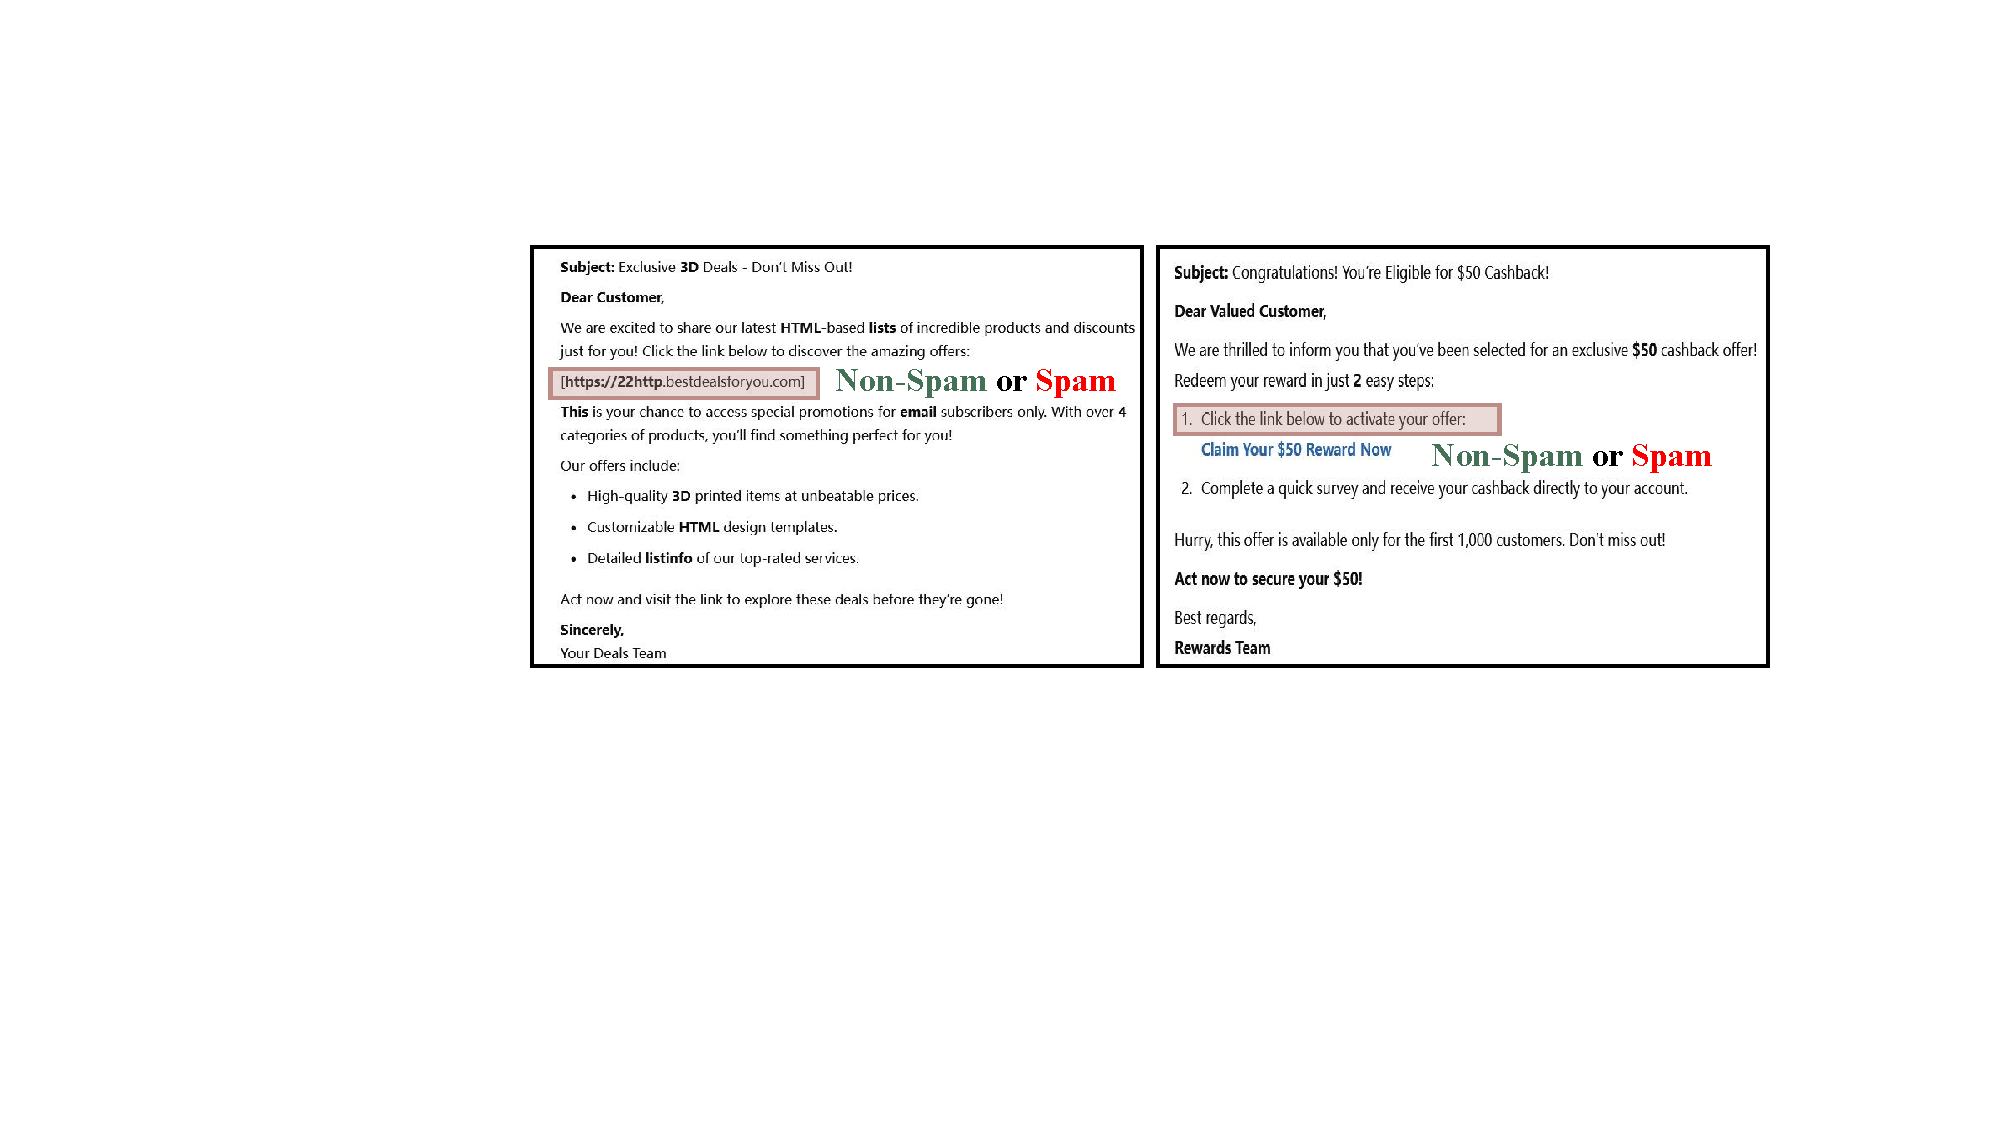
\includegraphics[keepaspectratio,height=3cm]{Graph/Evaluation/SPAM-Dynamics.pdf}
%	\caption{Uncertainty Dynamics in SPAM Email}
%	\label{fig:Uncertainty Dynamics for SPAM}
%\end{figure}
%We selected two feature vectors from spam emails in the SPAM dataset and used AIGC to generate corresponding email content.
%Whether identical feature vectors are classified as spam is not determined by the textual characteristics alone but rather by whether the embedded links are malicious.
%Attackers can exploit this by generating high-uncertainty samples with identical features but opposite labels. Such samples can significantly degrade the concept drift adaptation performance of the target model.
%For example, in spam detection, sample features are word vectors. 
%Using large language models (LLMs), attackers can generate poisoned samples with consistent features but flipped labels, adhering to the clean-label assumption through manual validation, as shown in Equation~\ref{EQ-Guided Untargeted Poisoning Attack}.
%\begin{equation}
%	\begin{aligned}
%		x_{seed}^{t+1} & = \max_{x_{p} \in D_{te}^{t}} uncer\left( x_{p+\alpha}, \theta_{t}^{*} \right)  \\
%		\text{s.t. } &
%		\begin{cases} 
%			uncer\left( x_{p+\alpha}, \theta_{t}^{*} \right)>\beta \\
%			y_{p+\alpha} \neq y_{p}
%		\end{cases}  \\
%	\end{aligned}
%	\label{EQ-Guided Untargeted Poisoning Attack}
%\end{equation}
%
%\subsection{Uncertainty Dynamics based on AIGC}
%\label{Sec: Uncertainty Dynamics based on LLM}
%With the help of generative models, attackers can perturb the uncertainty of existing samples at minimal cost.
%This is particularly significant in domains such as text, images, and videos, where the semantic meaning of labels evolves over time.
%\begin{figure}[htbp]
%	\centering
%	
\includegraphics[width=8cm,height=3cm]{Graph/Evaluation/Figure17-Bird.pdf}
%	\caption{Uncertainty Dynamics based on AIGC (Bird)}
%	\label{fig:Uncertainty Dynamics based on LLM}
%\end{figure}
%Attackers have substantial flexibility in these areas, as the real-world meanings of text and visual entities are constantly evolving.
%As shown in Figure~\ref{fig:Uncertainty Dynamics based on LLM} and Figure~\ref{fig:Uncertainty Dynamics based on LLM-Deer}, we leverage AIGC to quickly generate a series of images with gradually shifting concepts.
%As shown in Figure~\ref{fig:Uncertainty Dynamics based on LLM} and Figure~\ref{fig:Uncertainty Dynamics based on LLM-Deer}, we leverage AIGC to generate images with gradually shifting concepts quickly. 
%\begin{figure}[htbp]
%	\centering
%	
\includegraphics[width=8cm,height=3cm]{Graph/Evaluation/Figure17-deer.pdf}
%	\caption{Uncertainty Dynamics based on AIGC (Deer)}
%	\label{fig:Uncertainty Dynamics based on LLM-Deer}
%\end{figure}
%Attackers do not need to worry about label flipping, as high uncertainty is the core requirement for poisoned samples in \pandora attacks (UPA).
%Furthermore, our experiments on concept drift direction-guided untargeted attacks using the SPAM dataset (Figure~\ref{fig:Untargeted-Attack-Guided}) reveal that label flipping can even enhance the effectiveness of UPA attacks.

%\section{Attacker Cost Analysis}
%\label{Sec: Attacker Cost Analysis}
%
%\noindent The attacker’s cost structure is complicated, including manual labeling, poisoned seed sample search, and sample generation costs.
%Since the attacker’s surrogate model training phase uses pseudo labels, the active learning process has no manual labeling cost.
%The main labeling cost is used for the search of poisoned samples, which is much smaller than the annotation cost in the active learning process of the victim model, as the attacker only needs to focus on a small number of highly uncertain samples within each test cycle.
%Attackers need to pay a specific cost for the construction of poisoned samples.
%This part involves the construction of the corresponding problem space after the feature space is determined.  
%Large language models can assist attackers in constructing poisoned samples, such as poisoned images and text.
%The problem-space construction of malware samples is inherently more complex.
%However, there are also mature tools available to use~\cite{virboxprotector}.
%We tested mainstream tools and found that the average processing time was 75 seconds per sample.
%The average size of the samples is 199.72MB, and the sample list is shown in Table \ref{tab: APK obfuscation time}. 
%In addition to the fact that automated tools in the industry have significantly reduced the cost of constructing poisoned samples for attackers, existing academic research has shown that related construction is feasible, with the construction time for a single sample being 10 minutes~\cite{2023-CCS-Query-Based-Evasion-Attack}.
%
%\begin{table}[htbp]
%	\centering
%	\small
%	\renewcommand{\arraystretch}{0.8}
%	\caption{APK obfuscation Time}
%	%\renewcommand{\arraystretch}{0.8}  % 调整该表格的行距
%	\label{tab: APK obfuscation time}
%	\begin{tabular}{c|c|c}
%		\toprule
%		\textbf{APK} & \textbf{Size (MB)} & \textbf{Obfuscation time} \\
%		\midrule
%		JD & 97.59 & 54.95s \\
%		Taobao & 57.03 & 78.98s \\
%		Little Red Book & 162.99 & 178.68s \\
%		Google & 315.67 & 93.32s \\
%		Wang VPN & 45.51 & 14.91s \\
%		WeChat & 264.04 & 136.76s \\
%		\midrule
%		\textbf{Average} & 199.72 & 90.72s \\
%		\bottomrule
%	\end{tabular}
%\end{table} 

%\textcolor{blue}{The time overhead for the attacker is significantly less than the time required for model updating, therefore the attack can be successfully executed.}

%To fully demonstrate the rationality of attack in the problem space, we test the time cost of obfuscation operations.
%We aim to demonstrate that attackers can quickly map poisoned samples from the feature space to the problem space. We select APKs of different types and sizes. 
%Then, we test their repackaging and obfuscation time, as shown in Table \ref{tab: APK obfuscation time}. 
%Based on the time-based test result, we can observe that the average attack time overhead for a single sample in the problem space is less than 5 minutes. 
%Since the concept drift adaptation model is typically updated monthly, attackers have sufficient time to execute \pandora attacks.
% 从正文中摘出来的部分,也是时间开销相关的,整合到附录吧
%After fully confirming the effectiveness of the attack method, we conduct tests on the attack time cost, as shown in Table \ref{tab: Attack time cost}.
%We evaluat data from 2013 to 2018 and found that the current optimal concept drift adaptation method has an average feature space attack time cost of 5 minutes and 49 seconds. 
%Because of the different sizes of malware packages, the time cost for problem space attacks varies significantly.
%Therefore, we select various types of software, including e-commerce, gaming, and social media, to test the time cost of problem space attack operations. 
%The experimental results show that the average time cost for a single sample problem space attack operation is 6 minutes and 8 seconds. 
%In summary, the total time cost of the entire attack process is significantly lower than the model update frequency of mainstream concept drift adaptation methods.

%\begin{comment}
%	\begin{table*}[ht]
%		\centering
%		\small
%		\renewcommand{\arraystretch}{0.8}
%		\caption{\pandora Attack time cost}
%		\label{tab: Attack time cost}
%		\begin{tabular}{|c|*{12}{c|}}
%			\toprule
%			\multirow{3}{*}{Stage} & \multicolumn{12}{c|}{Concept Drift Strategy and Active Learning Label Budget} \\
%			\cmidrule{2-13}
%			& \multicolumn{6}{c|}{\textbf{CADE}} & \multicolumn{6}{c|}{\textbf{HCL}} \\
%			\cmidrule{2-13}
%			& 50 & 100 & 150 & 200 & 250 & 300 & 50 & 100 & 150 & 200 & 250 & 300 \\
%			\midrule
%			% 在此处插入表格数据
%			Seed Selection (Min) & 7.55 & 15.42 & 17.78 & 10.15 & 3.98 & 10.77 & 5.63 & 9.45 & 8.13 & 6.03 & 3.03 & 11.07 \\
%			Sample Generation (Min) & 1.7 & 3.58 & 4.37 & 2.08 & 1.47 & 5.52 & 1.23 & 2.52 & 2.27 & 1.85 & 1.07 & 4.35 \\
%			Model Update (Min) & 4.65 & 4.62 & 5.17 & 5.3 & 1.65 & 3.27 & 1.48 & 1.97 & 1.9 & 1.72 & 0.55 & 2.27\\
%			\midrule
%			\multirow{2}{*}{Stage} & \multicolumn{6}{c|}{\textbf{TRANS}} & \multicolumn{6}{c|}{\textbf{UNC}} \\
%			\cmidrule{2-13}
%			& 50 & 100 & 150 & 200 & 250 & 300 & 50 & 100 & 150 & 200 & 250 & 300 \\
%			\midrule
%			Seed Selection (Min) & 8.63 & 13.2 & 14.93 & 16.29 & 18.15 & 17.77 & 0.08 & 0.1 & 0.06 & 0.08 & 0.08 & 0.12 \\
%			Sample Generation (Min) & 2.52 & 2.63 & 2.82 & 3.05 & 3.17 & 2.57 & 0.1 & 0.03 & 0.03 & 0.03 & 0.1 & 0.2 \\
%			Model Update (Min) & 1.78 & 1.7 & 1.77 & 1.84 & 1.9 & 1.7 & 3.7 & 2.88 & 1.15 & 5.68 & 2.32 & 3.78 \\
%			\bottomrule
%		\end{tabular}
%	\end{table*}
%\end{comment}

%\subsection{Defence Parameter Analysis}
%\label{Sec: Defence Parameter Analysis}
%\noindent \textbf{Activation Clustering (AC)} is a data inspection method. 
%AC assumes the poisoned data in the target class forms a separate cluster that is either small or far from the class center.
%As shown in the Figure~\ref{fig:feature space entanglement}, we utilized the t-SNE tool to visualize the poisoned and non-poisoned samples.
%It can be observed that due to the \pandora attack's use of attack seeds for generating poisoned samples, there is a highly intricate entanglement between poisoned and non-poisoned samples in the feature space.
%As a result, poisoning defense methods based on the AC perform poorly.
%Not only do they fail to eliminate poisoned samples, but they also remove clean samples, thereby undermining the model's ability to generalize effectively.
%\noindent \textbf{(1) Feature Space Entanglement:} As shown in Figure~\ref{fig:feature space entanglement}, t-SNE visualization reveals that \pandora's use of attack seeds creates intricate entanglement between poisoned and clean samples in the feature space (the APIGraph dataset's test data from June 2013).
%Consequently, AC-based defences perform poorly, failing to remove poisoned samples while mistakenly eliminating clean ones, which weakens the model's generalization ability.
%\begin{figure}[htbp]
%	\centering
%	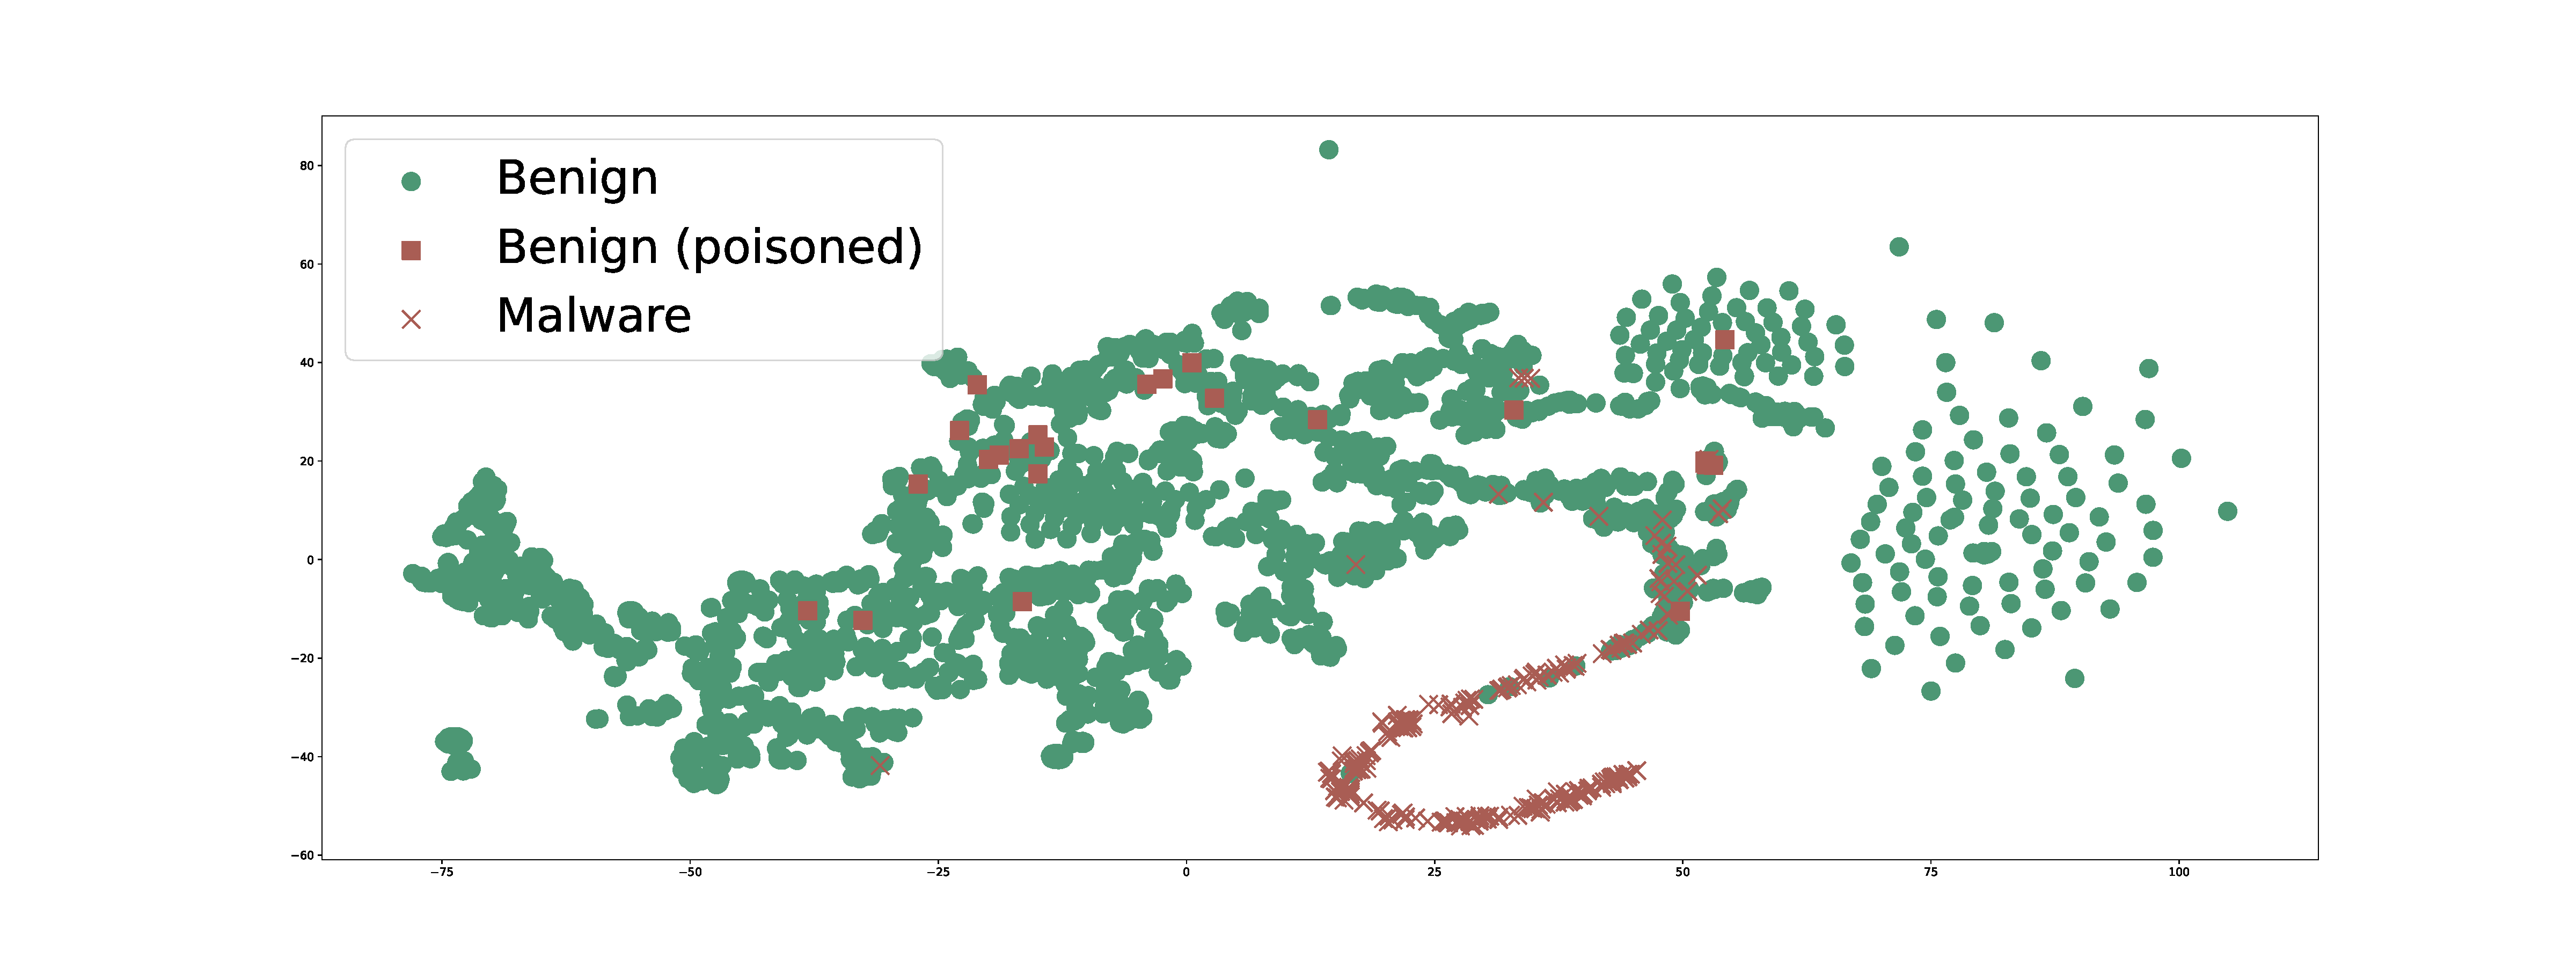
\includegraphics[width=\linewidth,keepaspectratio]{Graph/Evaluation/Figure24-v1}
%	\caption{Feature space entanglement}
%	\label{fig:feature space entanglement}
%\end{figure}
%Due to the longer time span of multi-target attack testing, we selected the APIGraph dataset for defense parameter analysis. 
%The number of clusters was the only parameter requiring manual configuration during the defense.
%We evaluated four cluster settings (6, 10, 20, and 40) under the multi-target attack. 
%The mean F1 score across these four settings was 0.91, with a variance of 0.0025.
%In the single-target attack, we selected the family 'clicks' (with the best ICDF defense performance) and the family 'mogap' (with the worst ICDF defense performance) from the Top 10 attack targets.
%For each family, we conducted four experiments with clustering parameter settings of 6, 10, 20, and 40 and observed that the defense performance remained consistent across all settings.
%This indicates that the defense parameter settings have minimal impact on defense effectiveness, which can effectively reduce the deployment costs of the defense method.

%\section{Practical Significance of \pandora}
%\label{Sec: Practical Significance of \pandora Attacks}
%Attackers can degrade the performance of target models, posing significant threats to the safety of real-world users.
%These risks are particularly severe in sensitive domains such as malware detection and industrial risk analysis, where attacks can lead to financial and physical harm to users.
%In the malware detection scenario studied in this paper, \pandora (under TPA) extends the misclassification duration of specific targets (malware), resulting in longer survival times in real-world scenarios.
%This prolonged survival exacerbates security threats.
%For example, the GriftHorse malware~\cite{GriftHorseMalware}, discovered in November 2020, leveraged subscription-based SMS services to generate 1.5 million USD to 4 million USD in monthly revenue, infecting over 10 million Android devices across 70+ countries.
%If the attacker combines the \pandora attack simultaneously, the harm of the above-mentioned security incident may be further expanded.
%Furthermore, the successful attack targets of \pandora serve as valuable references for attackers in designing future malware, significantly enhancing the efficiency of malware development and amplifying its potential harm.

%\section{Case Study}
%To verify the practicality of leveraging inference uncertainty in real-world machine learning models, we also tested publicly available machine learning services, specifically Baidu's object recognition system~\cite{Baidu-ImageRecognition}. 
%Ten categories from the CIFAR-10 dataset were selected for evaluation.
%Image recognition models show lower uncertainty with single-concept images but higher uncertainty with multi-concept images.
%To explore this, we created conceptual combinations using GAI technologies, enabling attackers to manipulate sample uncertainty in mature machine-learning products.
%The images were generated by progressively increasing the number of conceptual elements, ranging from 1 to 10, with subsequent images incorporating more concepts.
%For detailed information about the images, please refer to Appendix~\ref{Sec: Uncertainty Dynamics based on LLM}.
%\begin{figure}[htbp]
%	\centering
%	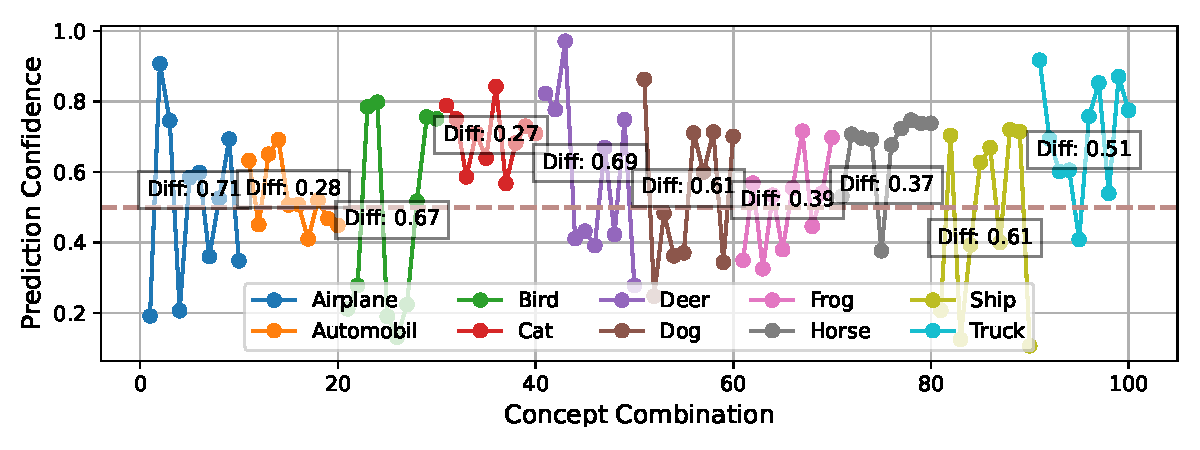
\includegraphics[width=\linewidth,keepaspectratio]{Graph/Evaluation/Figure18.pdf}
%	\caption{Case Study of Uncertainty Dynamics}
%	\label{fig:Case Study of Uncertainty Dynamics}
%\end{figure}
%Figure~\ref{fig:Case Study of Uncertainty Dynamics} illustrates notable fluctuations in sample uncertainty as additional concepts are introduced, with an average range of 0.511 between the highest and lowest uncertainty scores.
%Specifically, 90\% of test categories display uncertainty scores above 0.5 during conceptual combination tests, underscoring the vulnerability of mature machine learning models to manipulations in uncertainty.

%\subsection{Open Science}
%\label{Sec: Open Science}
%\noindent In order to enhance the reproducibility and replicability of scientific findings, we will share our research artifacts. 
%Our code (\url{}) and CDAMAL dataset (\url{https://anonymous.4open.science/r/CDAMAL-Concept-Drift-Dataset-3E08}) are all available. 
%In addition, considering research ethics, our dataset and the source code of the \pandora attack will only share minimized demonstration examples by default to illustrate the attack's effectiveness.